\section{Elevator Maintenance Planning and Scheduling}

\begin{frame}
\frametitle{Joint work with...}
\begin{itemize}
\item Mark Antunes, Vincent Armant, Kenneth N. Brown, Gabriel G. Castane, Daniel Desmond,
Guillaume Escamocher, Michele Garraffa, Anne-Marie George, Diarmuid Grimes, Mike O'Keefe, Yiqing Lin,
Barry O'Sullivan, Cemalettin Ozturk, Luis Quesada, Mohamed Siala, Helmut Simonis
and Nic Wilson
\end{itemize}
\end{frame}

\subsection{Introduction}

\begin{frame}
\frametitle{Real World Problem}
\begin{itemize}
\item Manufacturing Industry, after sales support
\item Maintenance is crucial for safety/availability of product
\item Preventive/Predictive/Reactive Maintenance influence each other
\item  How to organize service, what to do?
\end{itemize}
\end{frame}

\begin{frame}
\frametitle{Research Challenge}
\begin{itemize}
\item How to plan/schedule if events interrupt planned work
\item How to use predictive maintenance to avoid problems before they occur
\item What is the right problem decomposition?
\end{itemize}
\end{frame}

% \begin{frame}
% \frametitle{Using Industrial Problems as Research Challenge}
% \begin{itemize}
% \item Trying to make three points:
% \begin{itemize}
% \item This is an important industrial problem
% \item There is an interesting research question to be solved
% \item We are making a contribution to solving the problem
% \end{itemize}
% \item Highlighting some of the challenges
% \begin{itemize}
% \item Private data
% \item Scalability
% \item Managing expectations
% \end{itemize}
% \end{itemize}
% \end{frame}

\begin{frame}
\frametitle{Travelling Repair Person (TRP)}
\begin{itemize}
\item Providing service for devices at customer premises
\item Planned preventive maintenance and testing, regular visits
\item Technicians travel to multiple, but few customers per day
\item Unplanned repair work after faults, response-time critical
\item Service times quite variable
\item Impact of skills and local knowledge
\end{itemize}
\end{frame}

% \begin{frame}
% \frametitle{Compared to Other Service Planning Problems}
% \begin{itemize}
% \item Stationary technician, moving customers
% \begin{itemize}
% \item Example: car tune-up
% \item Preventive, planned work
% \item Either a queuing or scheduling problem
% \end{itemize}
% \item Moving customer, moving technician
% \begin{itemize}
% \item Road side assistance
% \item Reactive, unplanned work
% \item On-line dispatching, pre-positioning
% \end{itemize}
% \item Moving technician, stationary customers
% \begin{itemize}
% \item Example: cable installation, photocopier repair
% \item Mainly reactive, sometimes planned work as well
% \item Routing and scheduling aspects
% \end{itemize}
% \end{itemize}
% \end{frame}

\begin{frame}
\frametitle{Why is this important? (1)}
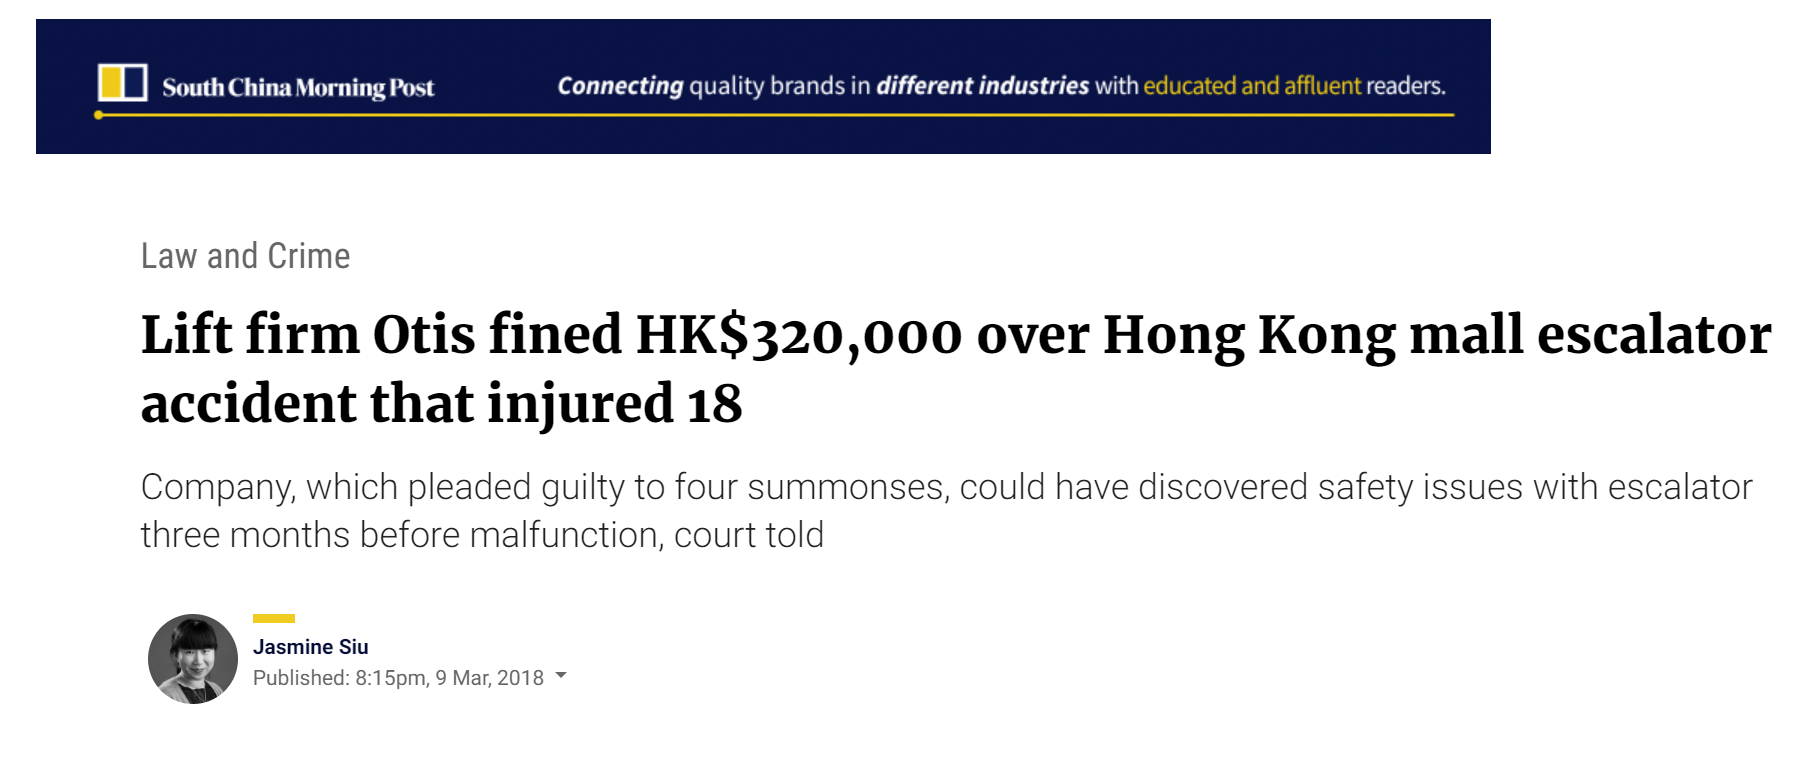
\includegraphics[width=11cm]{imagesfieldservice/southchina}
\end{frame}

\begin{frame}
\frametitle{Why is this important? (2)}
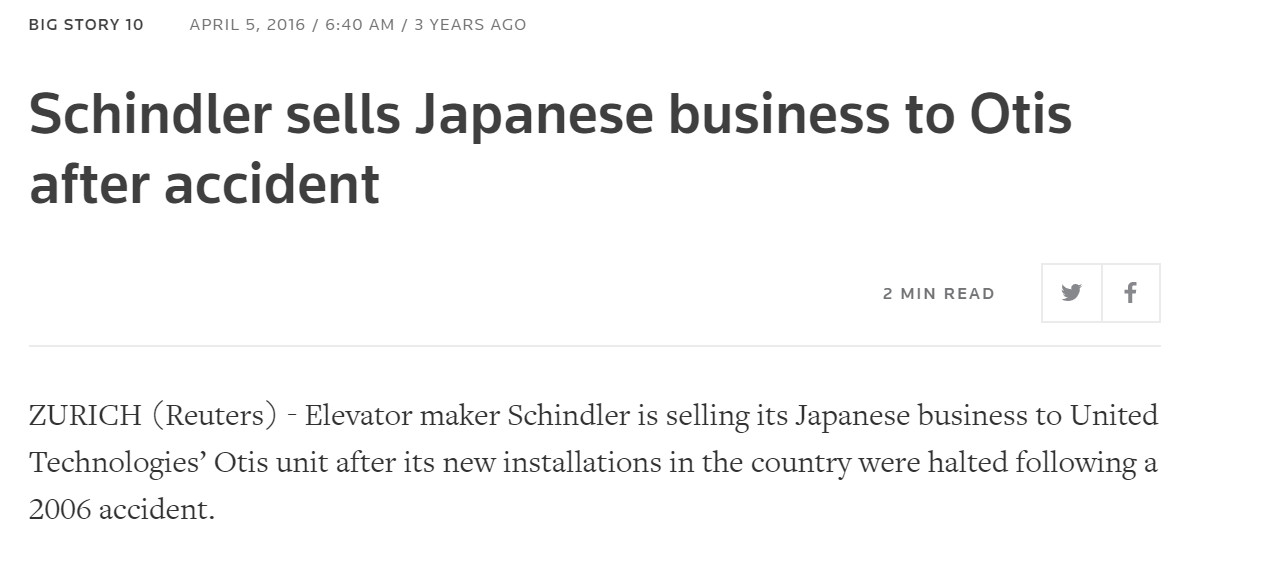
\includegraphics[width=11cm]{imagesfieldservice/schindlerjapan}

Source: 
\includegraphics[width=2cm]{imagesfieldservice/reuters}

\end{frame}

\begin{frame}
\frametitle{Why is this important? (3)}

\includegraphics[width=8cm]{imagesfieldservice/hancock}
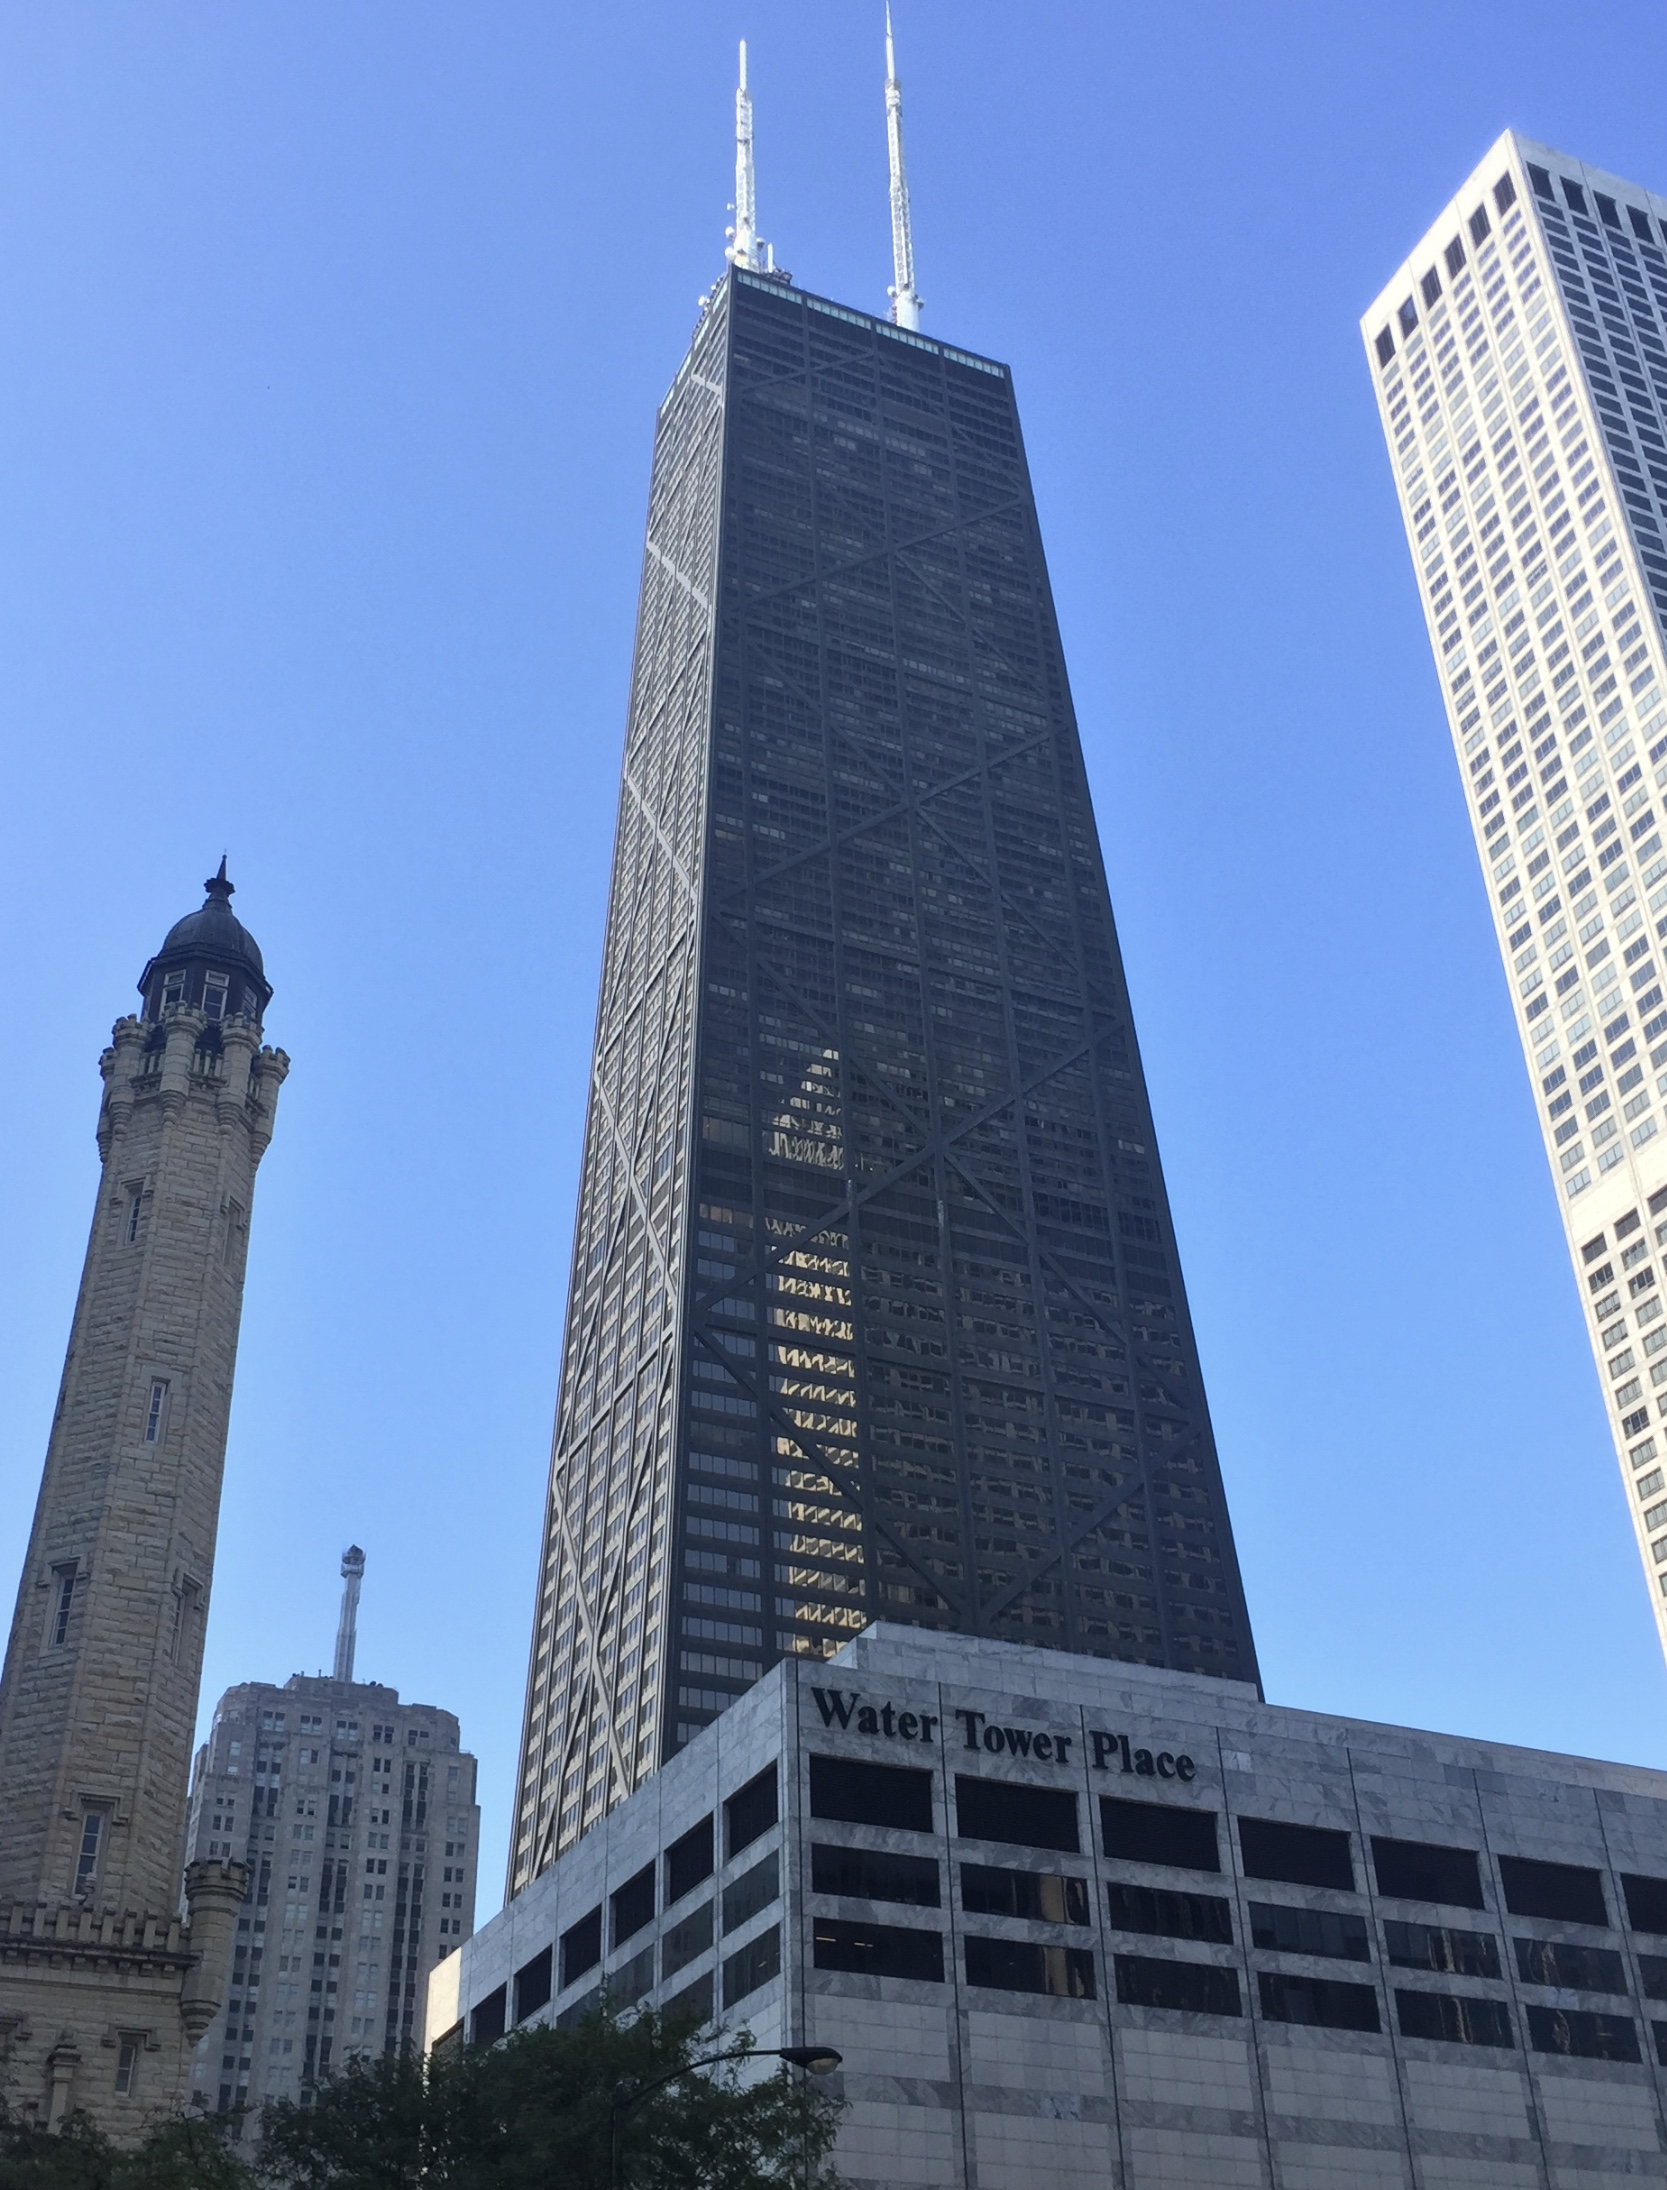
\includegraphics[width=3cm]{imagesfieldservice/John_Hancock_Center_2019}

{\tiny Source: By Chris6d - Own work, CC BY-SA 4.0, https://commons.wikimedia.org/w/index.php?curid=78201640}
\end{frame}

% \begin{frame}
% \frametitle{Why is this important? (4)}
% 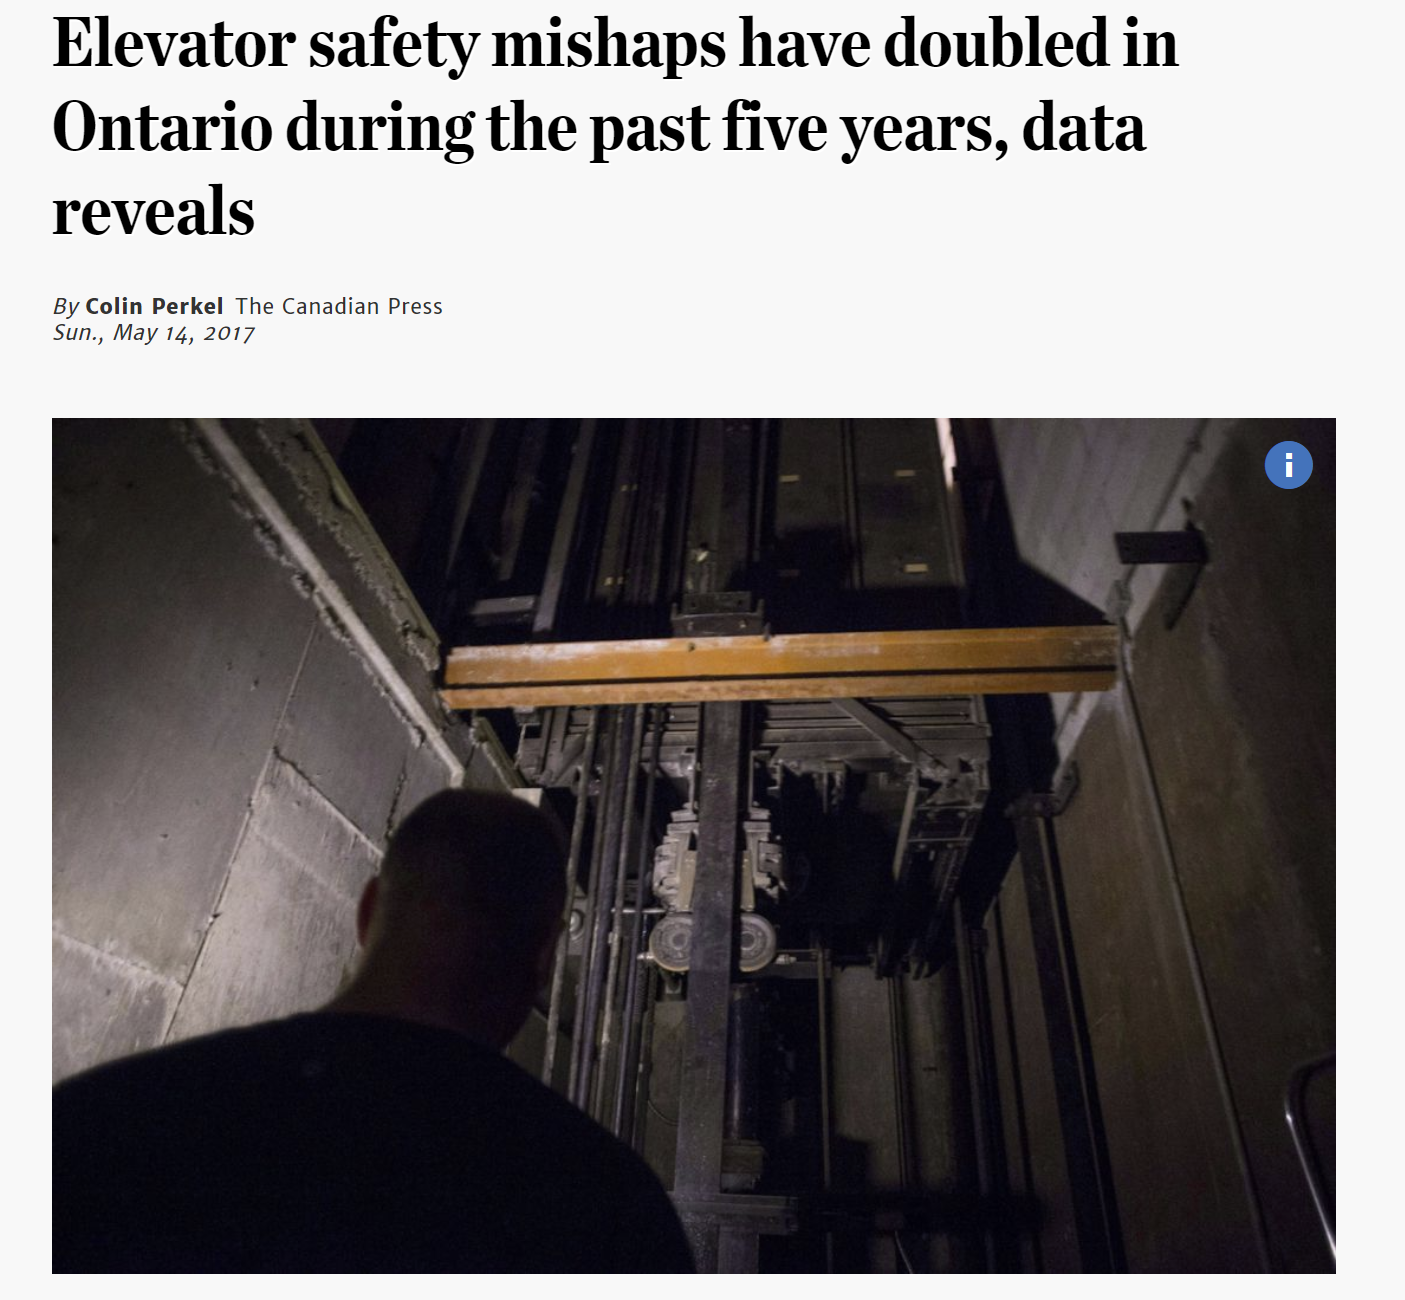
\includegraphics[width=7.5cm]{imagesfieldservice/ontario}
% \end{frame}


% \begin{frame}
% \frametitle{TRP Compared to Other Combinatorial Problems}
% 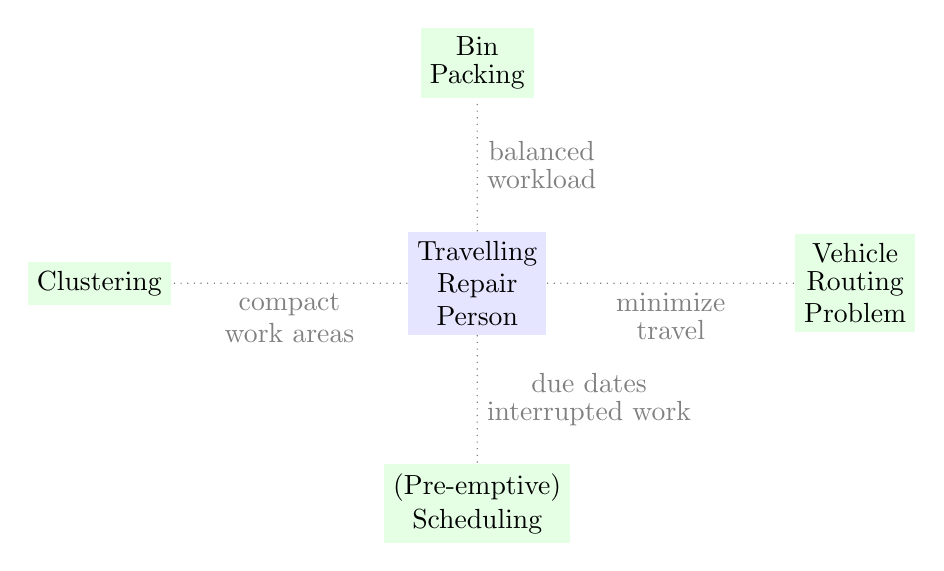
\begin{tikzpicture}[xscale=2.4,yscale=1.4]
  \node[fill=blue!10] (trp) at (2,2) {\shortstack{Travelling\\Repair\\Person}};
  \node[fill=green!10] (bin) at (2,4) {\shortstack{Bin\\Packing}};
  \node[fill=green!10] (clustering) at (0,2) {Clustering};
  \node[fill=green!10] (vrp) at (4,2) {\shortstack{Vehicle\\Routing\\Problem}};
  \node[fill=green!10] (scheduling) at (2,0) {\shortstack{(Pre-emptive)\\Scheduling}};
  \draw[gray,dotted] (trp) -- node[right] {\shortstack{balanced\\workload}} (bin);
  \draw[gray,dotted] (trp) -- node[below] {\shortstack{compact\\work areas}}(clustering);
  \draw[gray,dotted] (trp) -- node[below] {\shortstack{minimize\\travel}} (vrp);
  \draw[gray,dotted] (trp) -- node[right] {\shortstack{due dates\\interrupted work}} (scheduling);
\end{tikzpicture}

% \end{frame}

% \begin{frame}
% \frametitle{TRP - Interesting Research Problem}
% \begin{itemize}
% \item Combines elements of multiple combinatorial problems
% \item Hard constraints, multiple cost element
% \item Stochastic events are core part of problem
% \end{itemize}
% \end{frame}

% \begin{frame}
% \frametitle{Key Research Challenge}
% \begin{itemize}
% \item Use combination of Optimization and Simulation to model and solve the TRP
% \item Optimization
% \begin{itemize}
% \item Good for global cost model
% \item Detailed constraints of problem
% \item (-) Does not easily deal with unplanned work
% \end{itemize}
% \item Simulation
% \begin{itemize}
% \item Good for modelling individual actors
% \item Understanding impact of stochastic changes
% \item (-) No global view of problem
% \end{itemize}
% \end{itemize}
% \end{frame}

\subsection{Our Contribution}

\begin{frame}
\frametitle{High-level View}
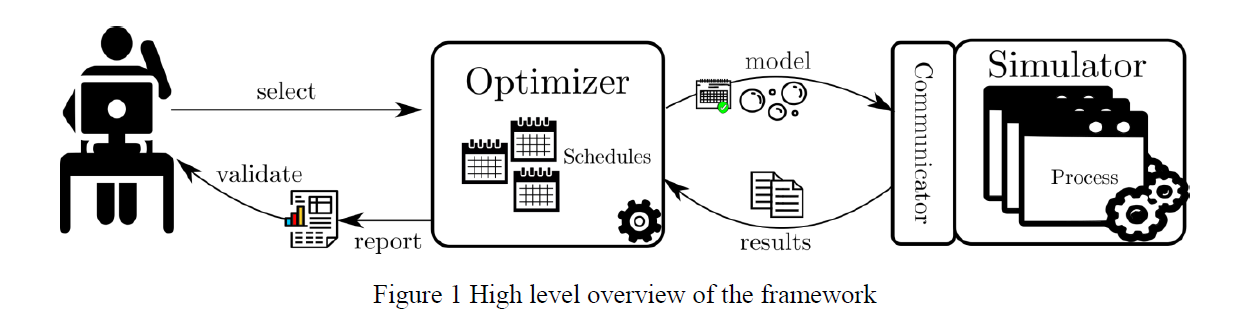
\includegraphics[width=11cm]{imagesfieldservice/highleveloverview}
\begin{itemize}
\item Optimizer deals with planning, load balancing, efficient schedules
\item Simulator explores how to react to changes
\item Simulator also provides one result as assumed reality
\end{itemize}
\end{frame}

\begin{frame}
\frametitle{Optimizer Design}
\begin{itemize}
\item Infeasible to build homogenuous model for complete problem
\item Added business process constraint
\begin{itemize}
\item Technicians should be responsible for ``their'' buildings
\item Improves service quality
\item Customers see familiar face
\end{itemize}
\item All work in one building should be performed by the same engineer, if possible
\item Engineers should be assigned compact areas of work
\item Balanced workload within the same depot
\end{itemize}
\end{frame}

\begin{frame}
\frametitle{Optimizer Decomposition}
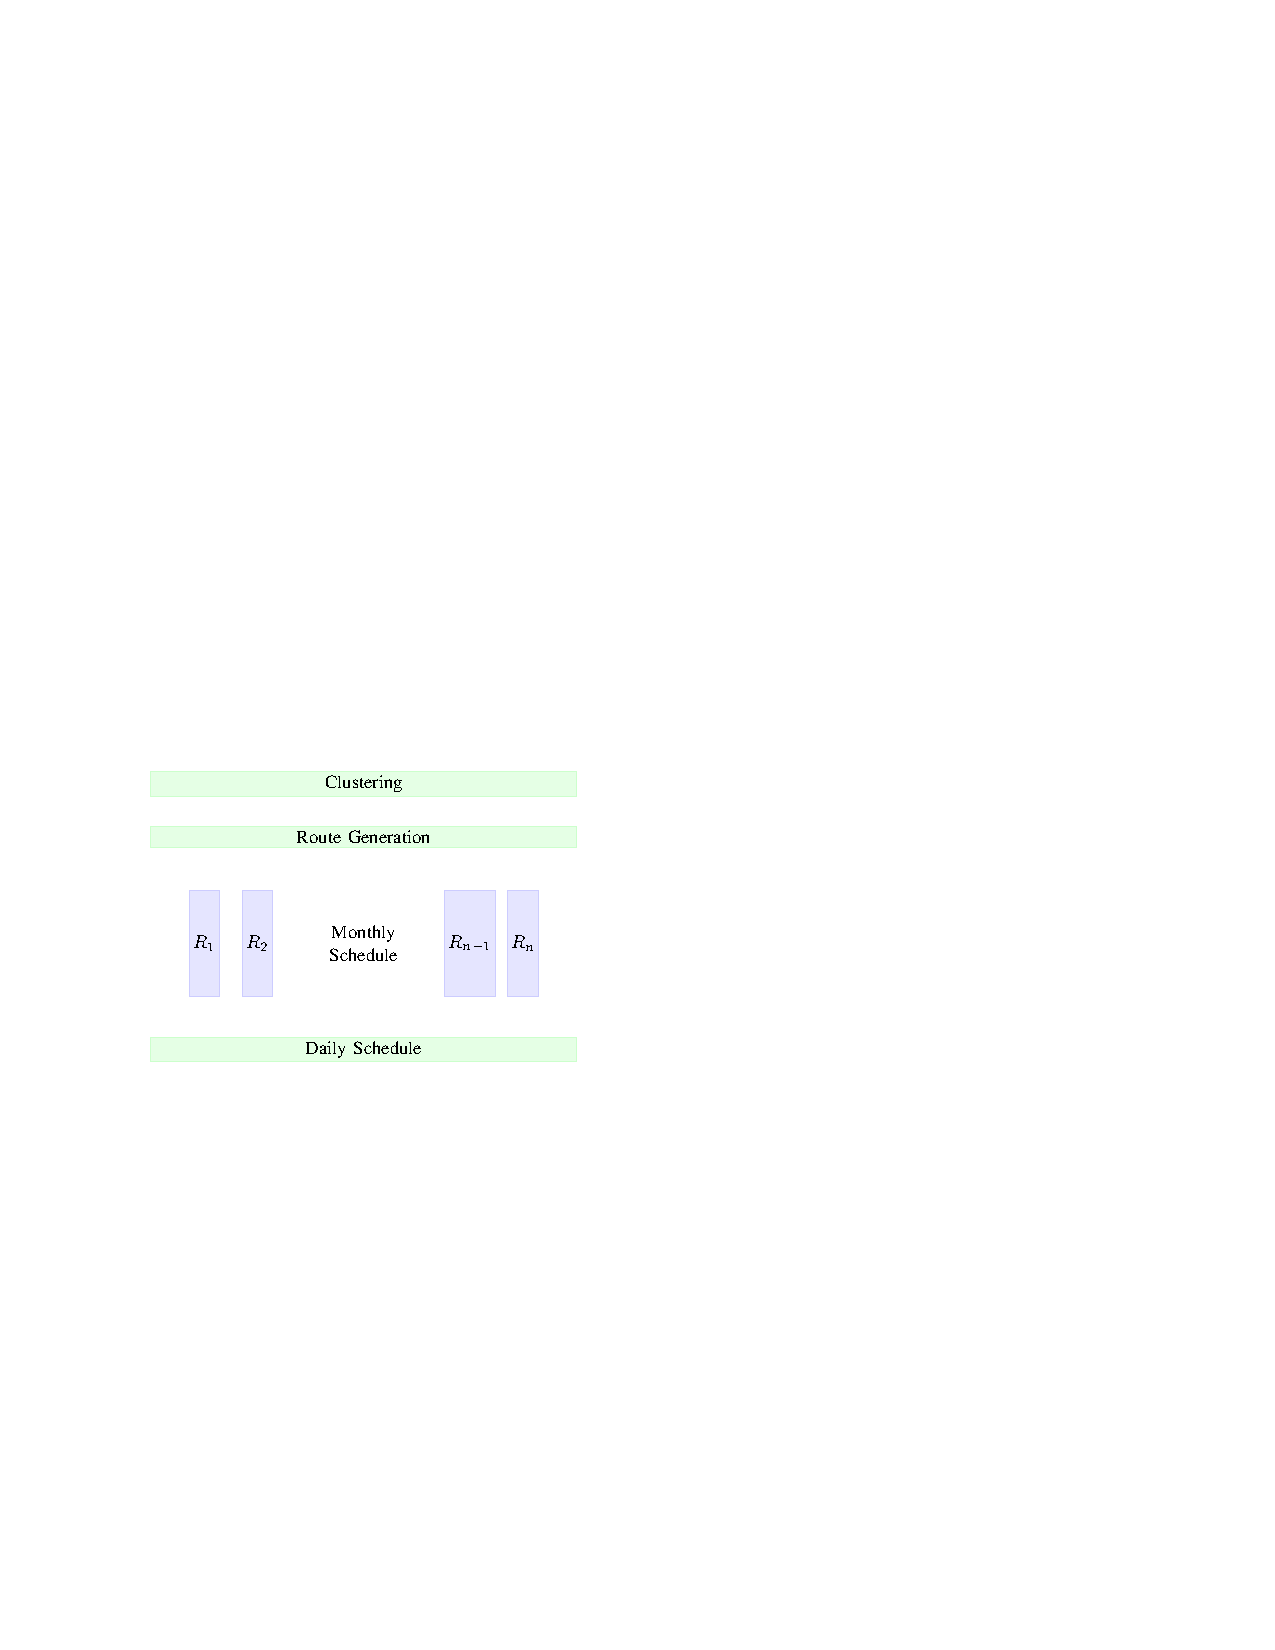
\includegraphics[width=10.5cm]{imagesfieldservice/decomposition}
\end{frame}

\begin{frame}
\frametitle{Clustering and Depot Assignment}
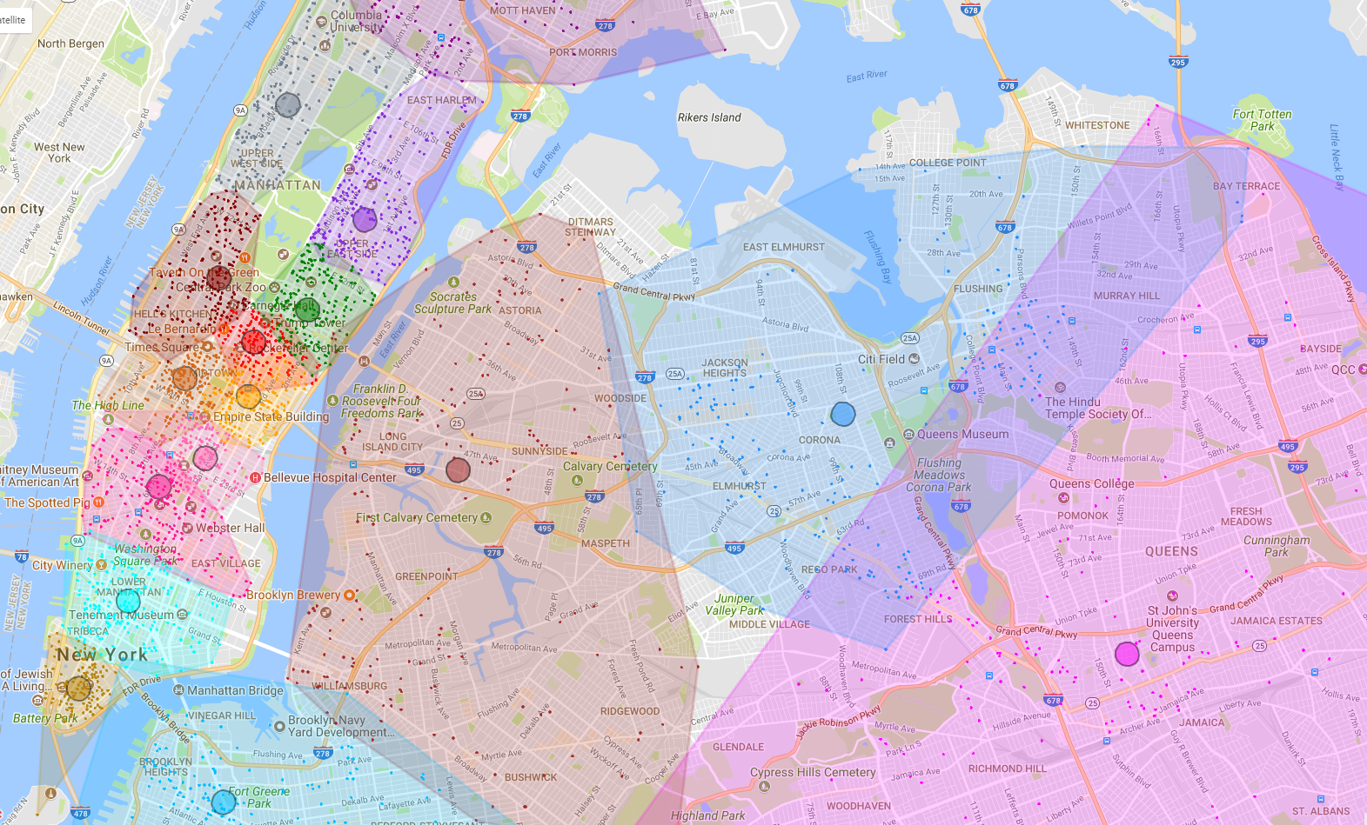
\includegraphics[width=11cm]{imagesfieldservice/depotassignment}
\end{frame}

% \begin{frame}
% \frametitle{Routes and Trips}
% 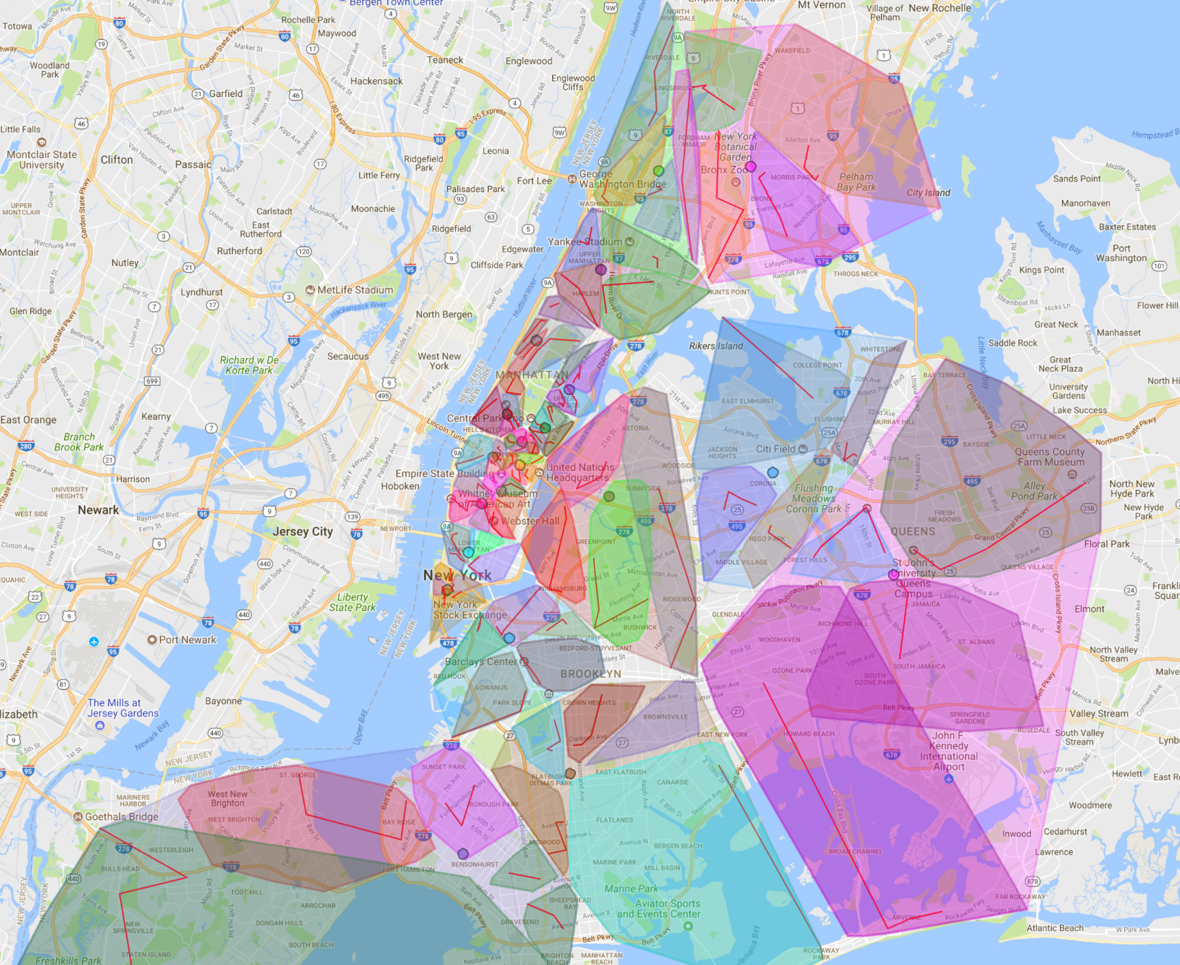
\includegraphics[width=8.5cm]{imagesfieldservice/toursinroutes}
% \end{frame}

% \begin{frame}
% \frametitle{Actual Data: Workload and Callbacks as Treemap}
% 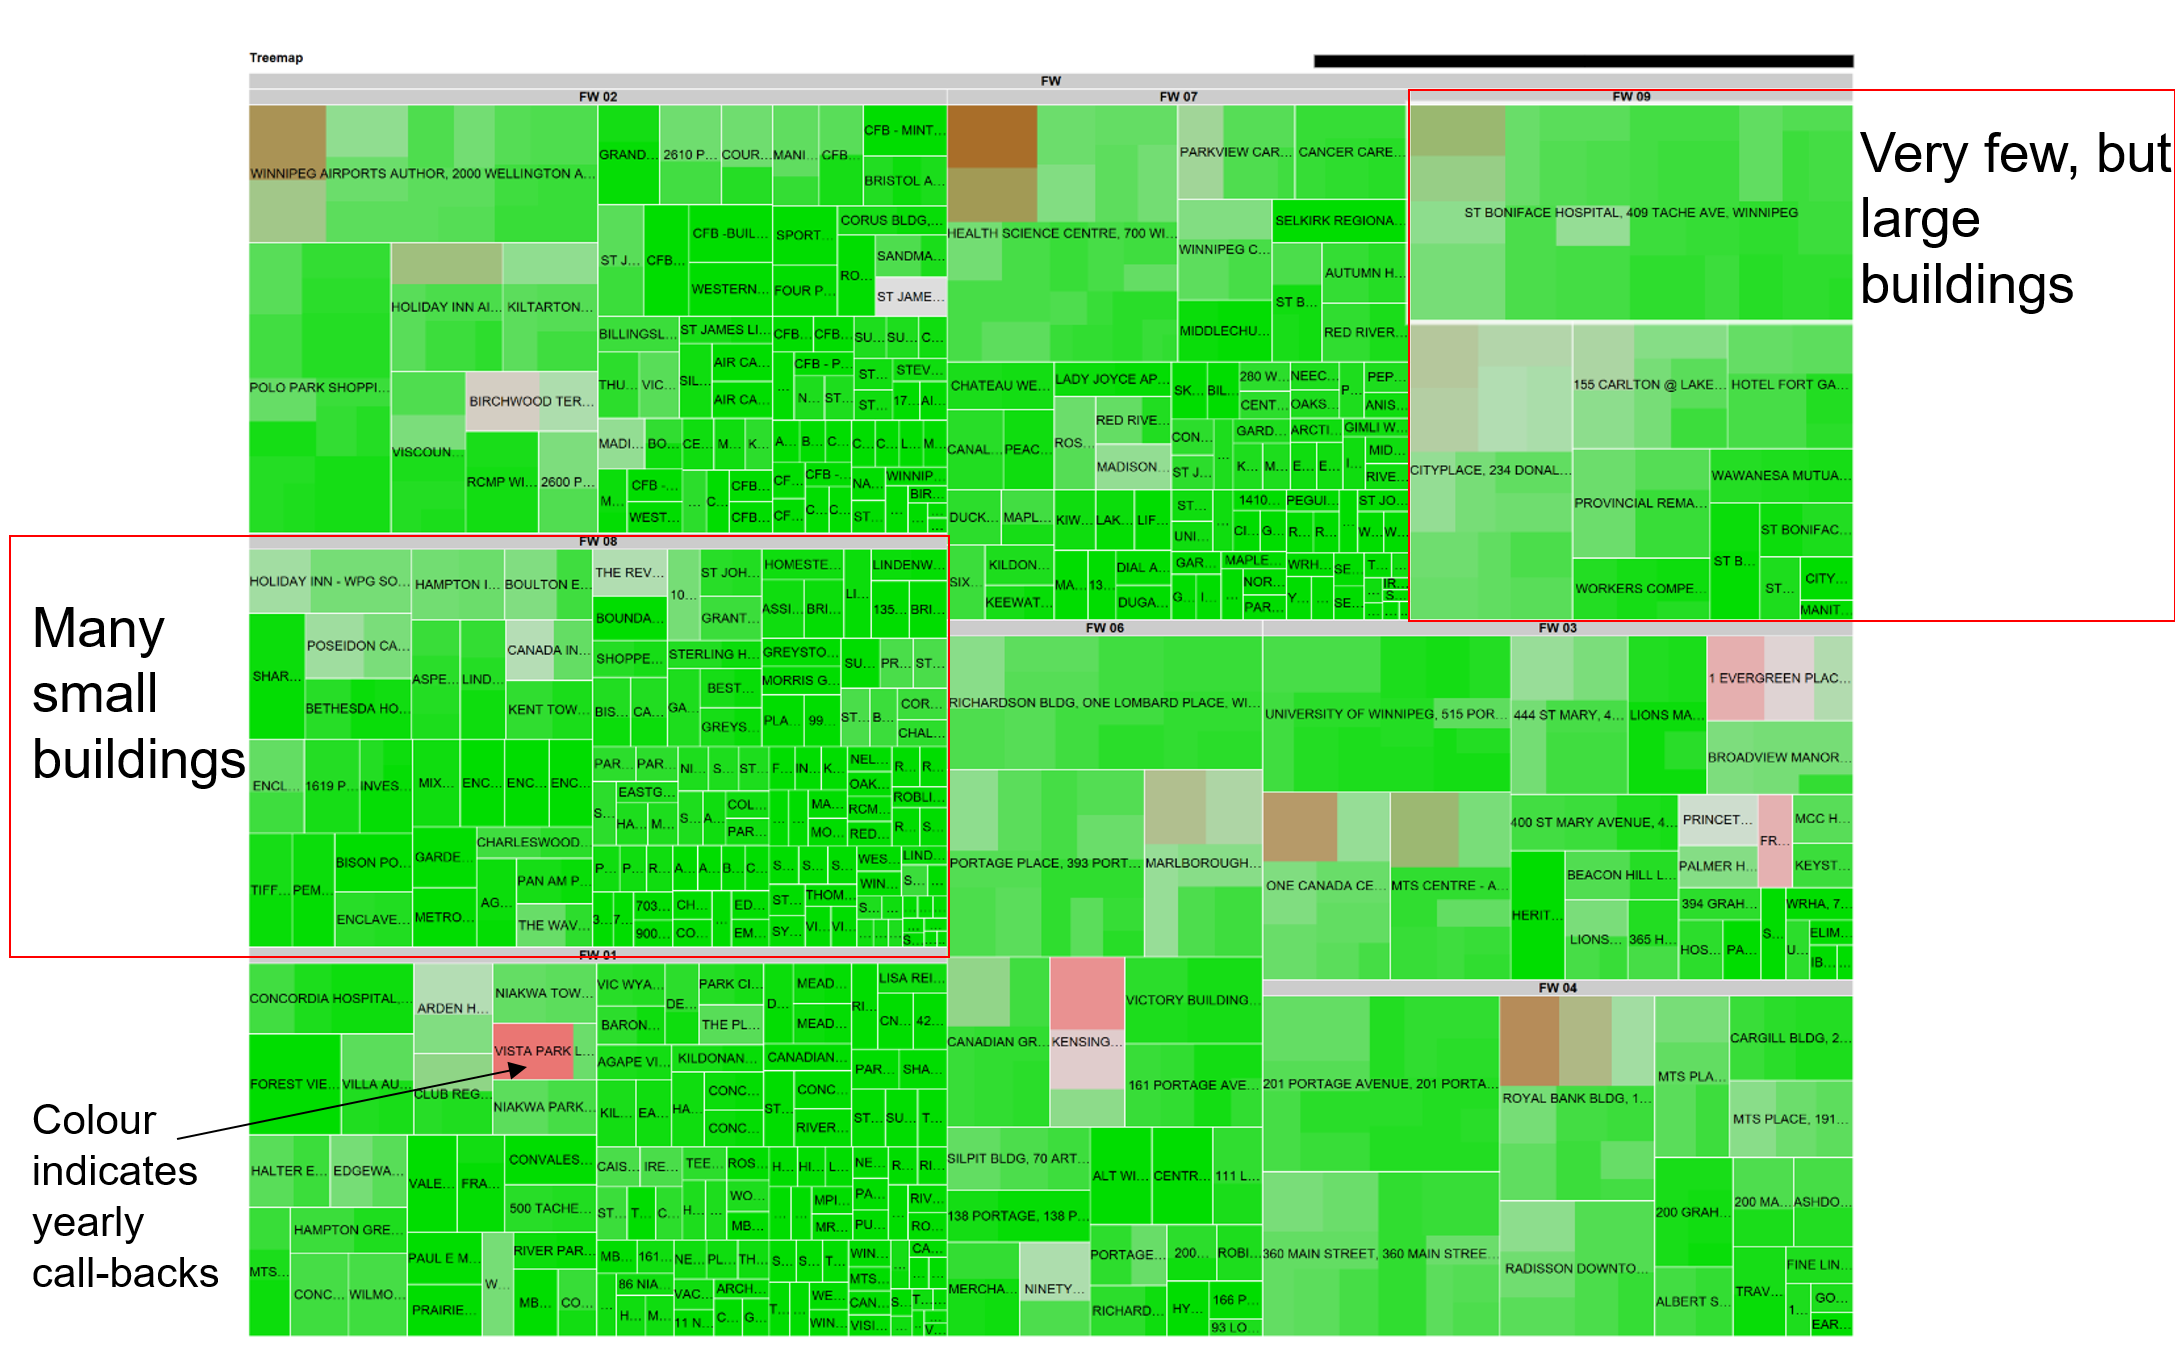
\includegraphics[width=11cm]{imagesfieldservice/treemap}
% \end{frame}

% \begin{frame}
% \frametitle{Actual Data: Mix of Urban and Rural Customers}
% 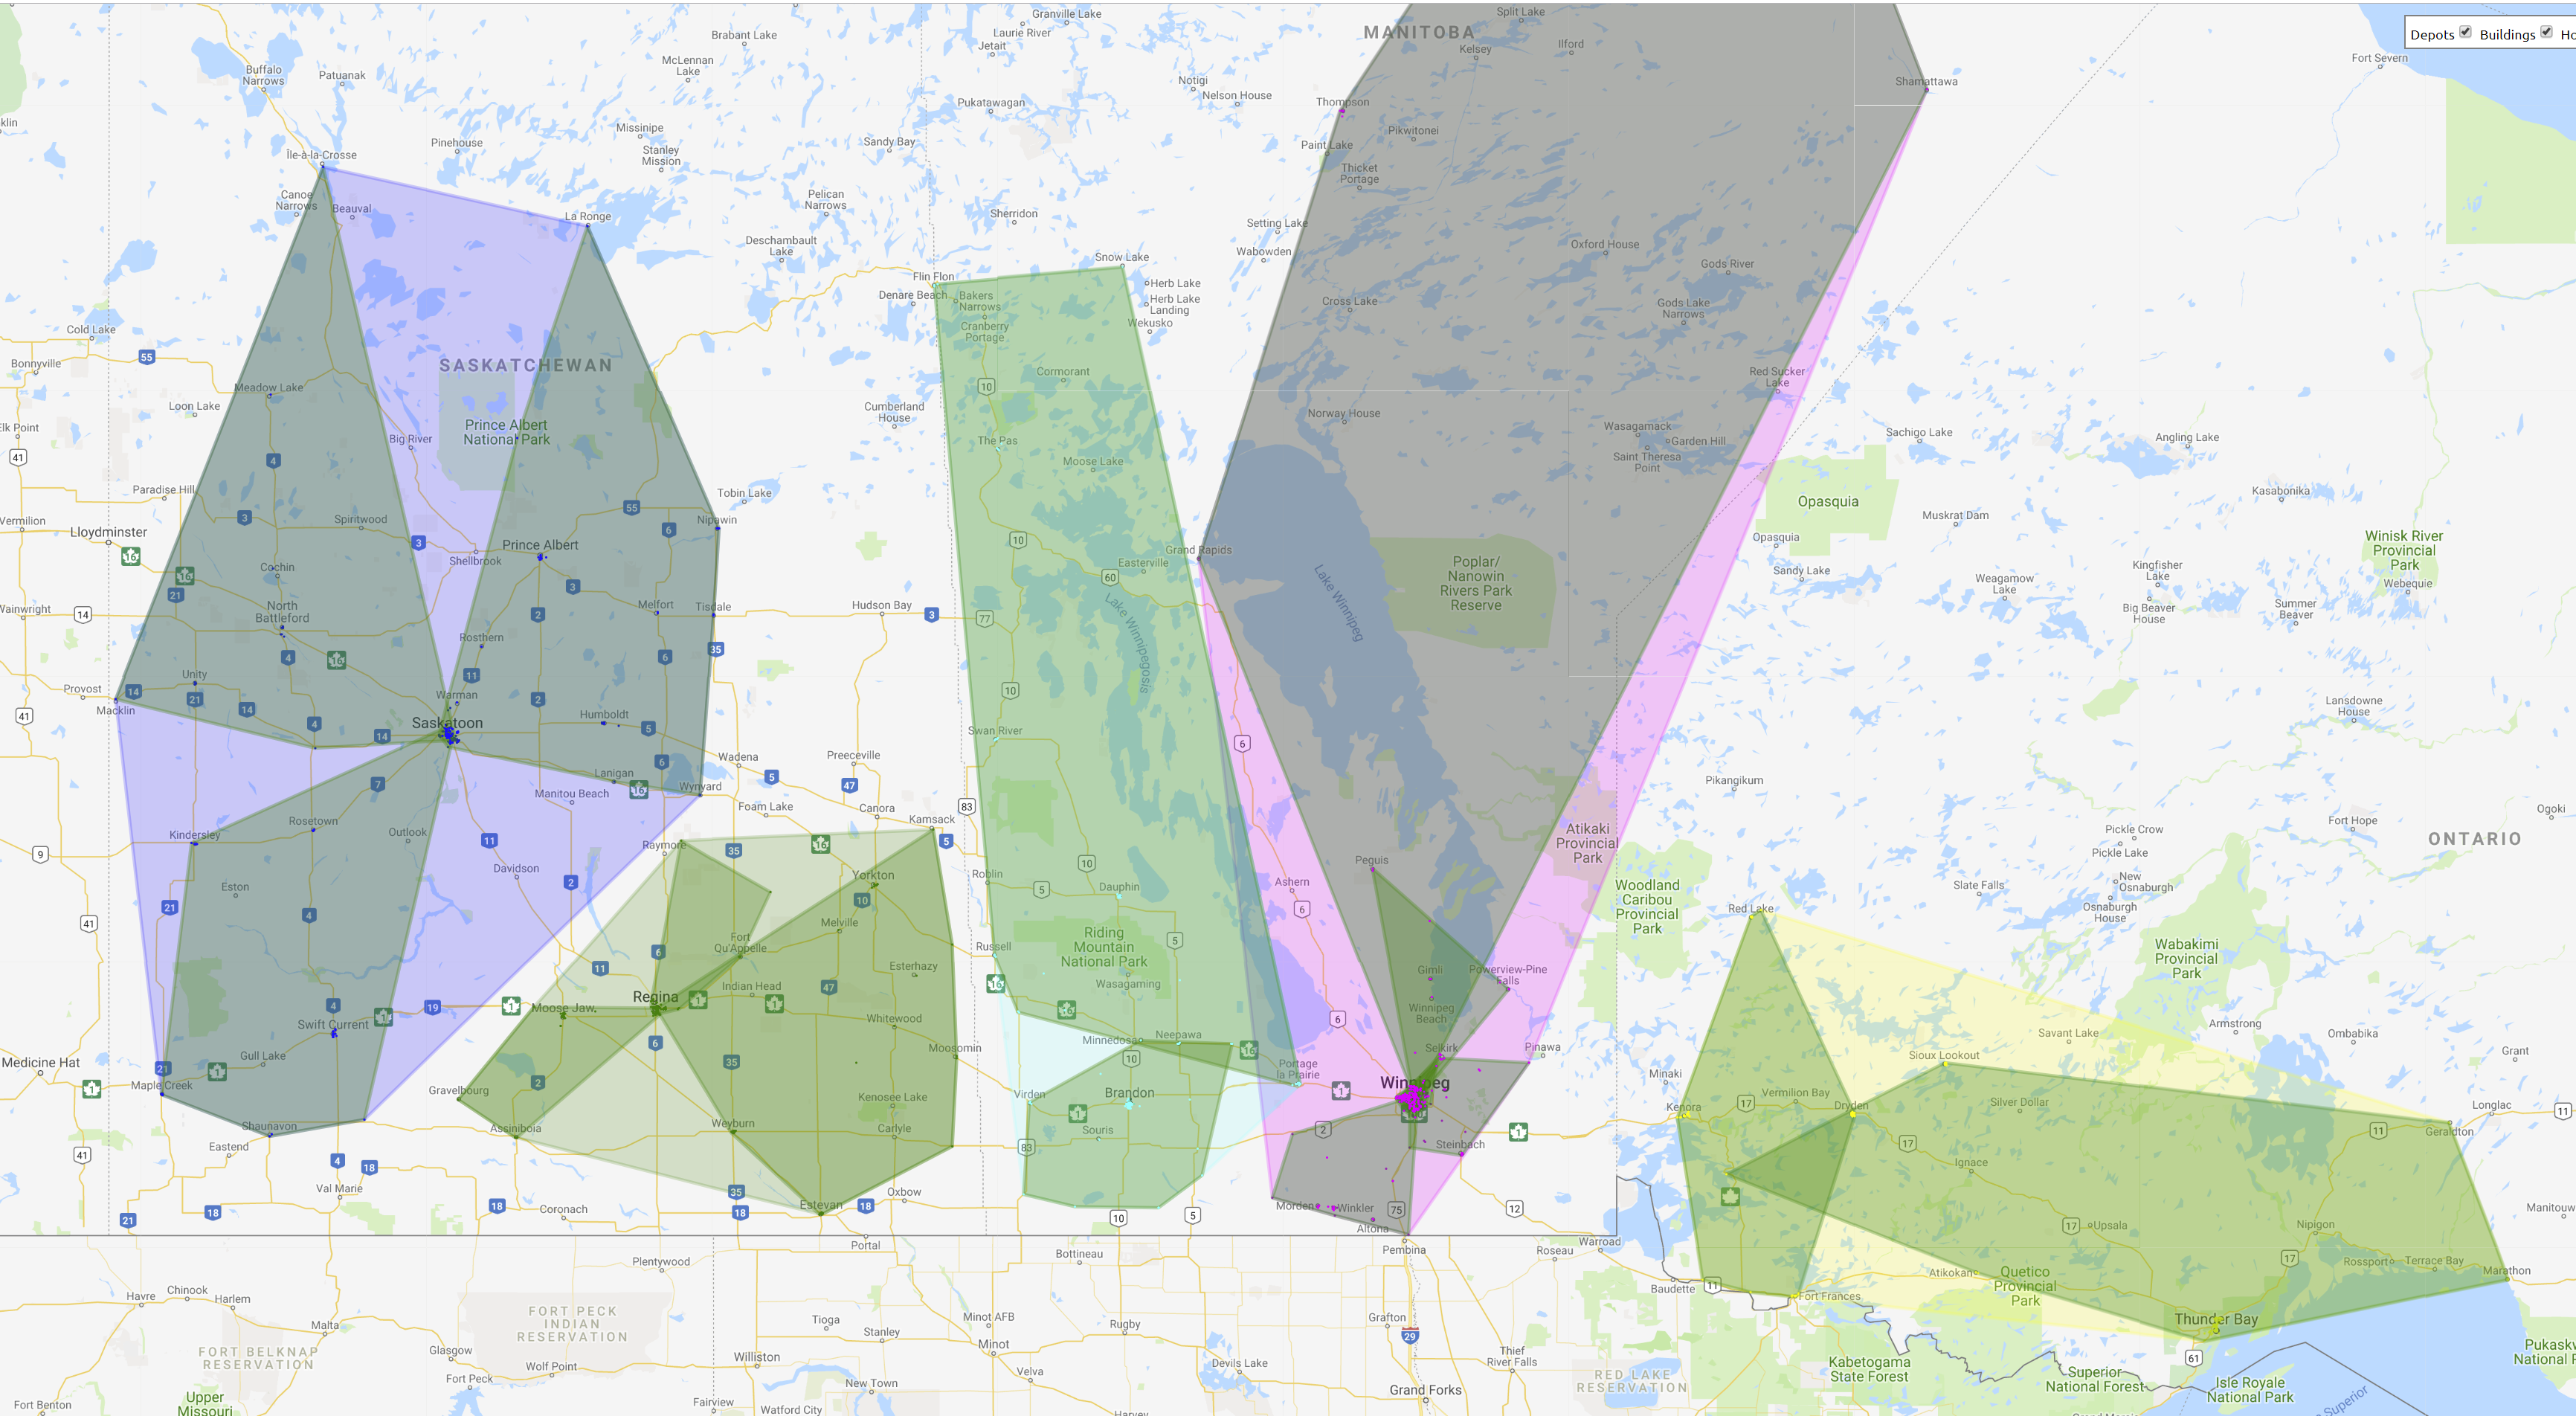
\includegraphics[width=11cm]{imagesfieldservice/mapcanada}
% \end{frame}

% \begin{frame}
% \frametitle{Actual Data: Balancing Workload Within Depots}
% 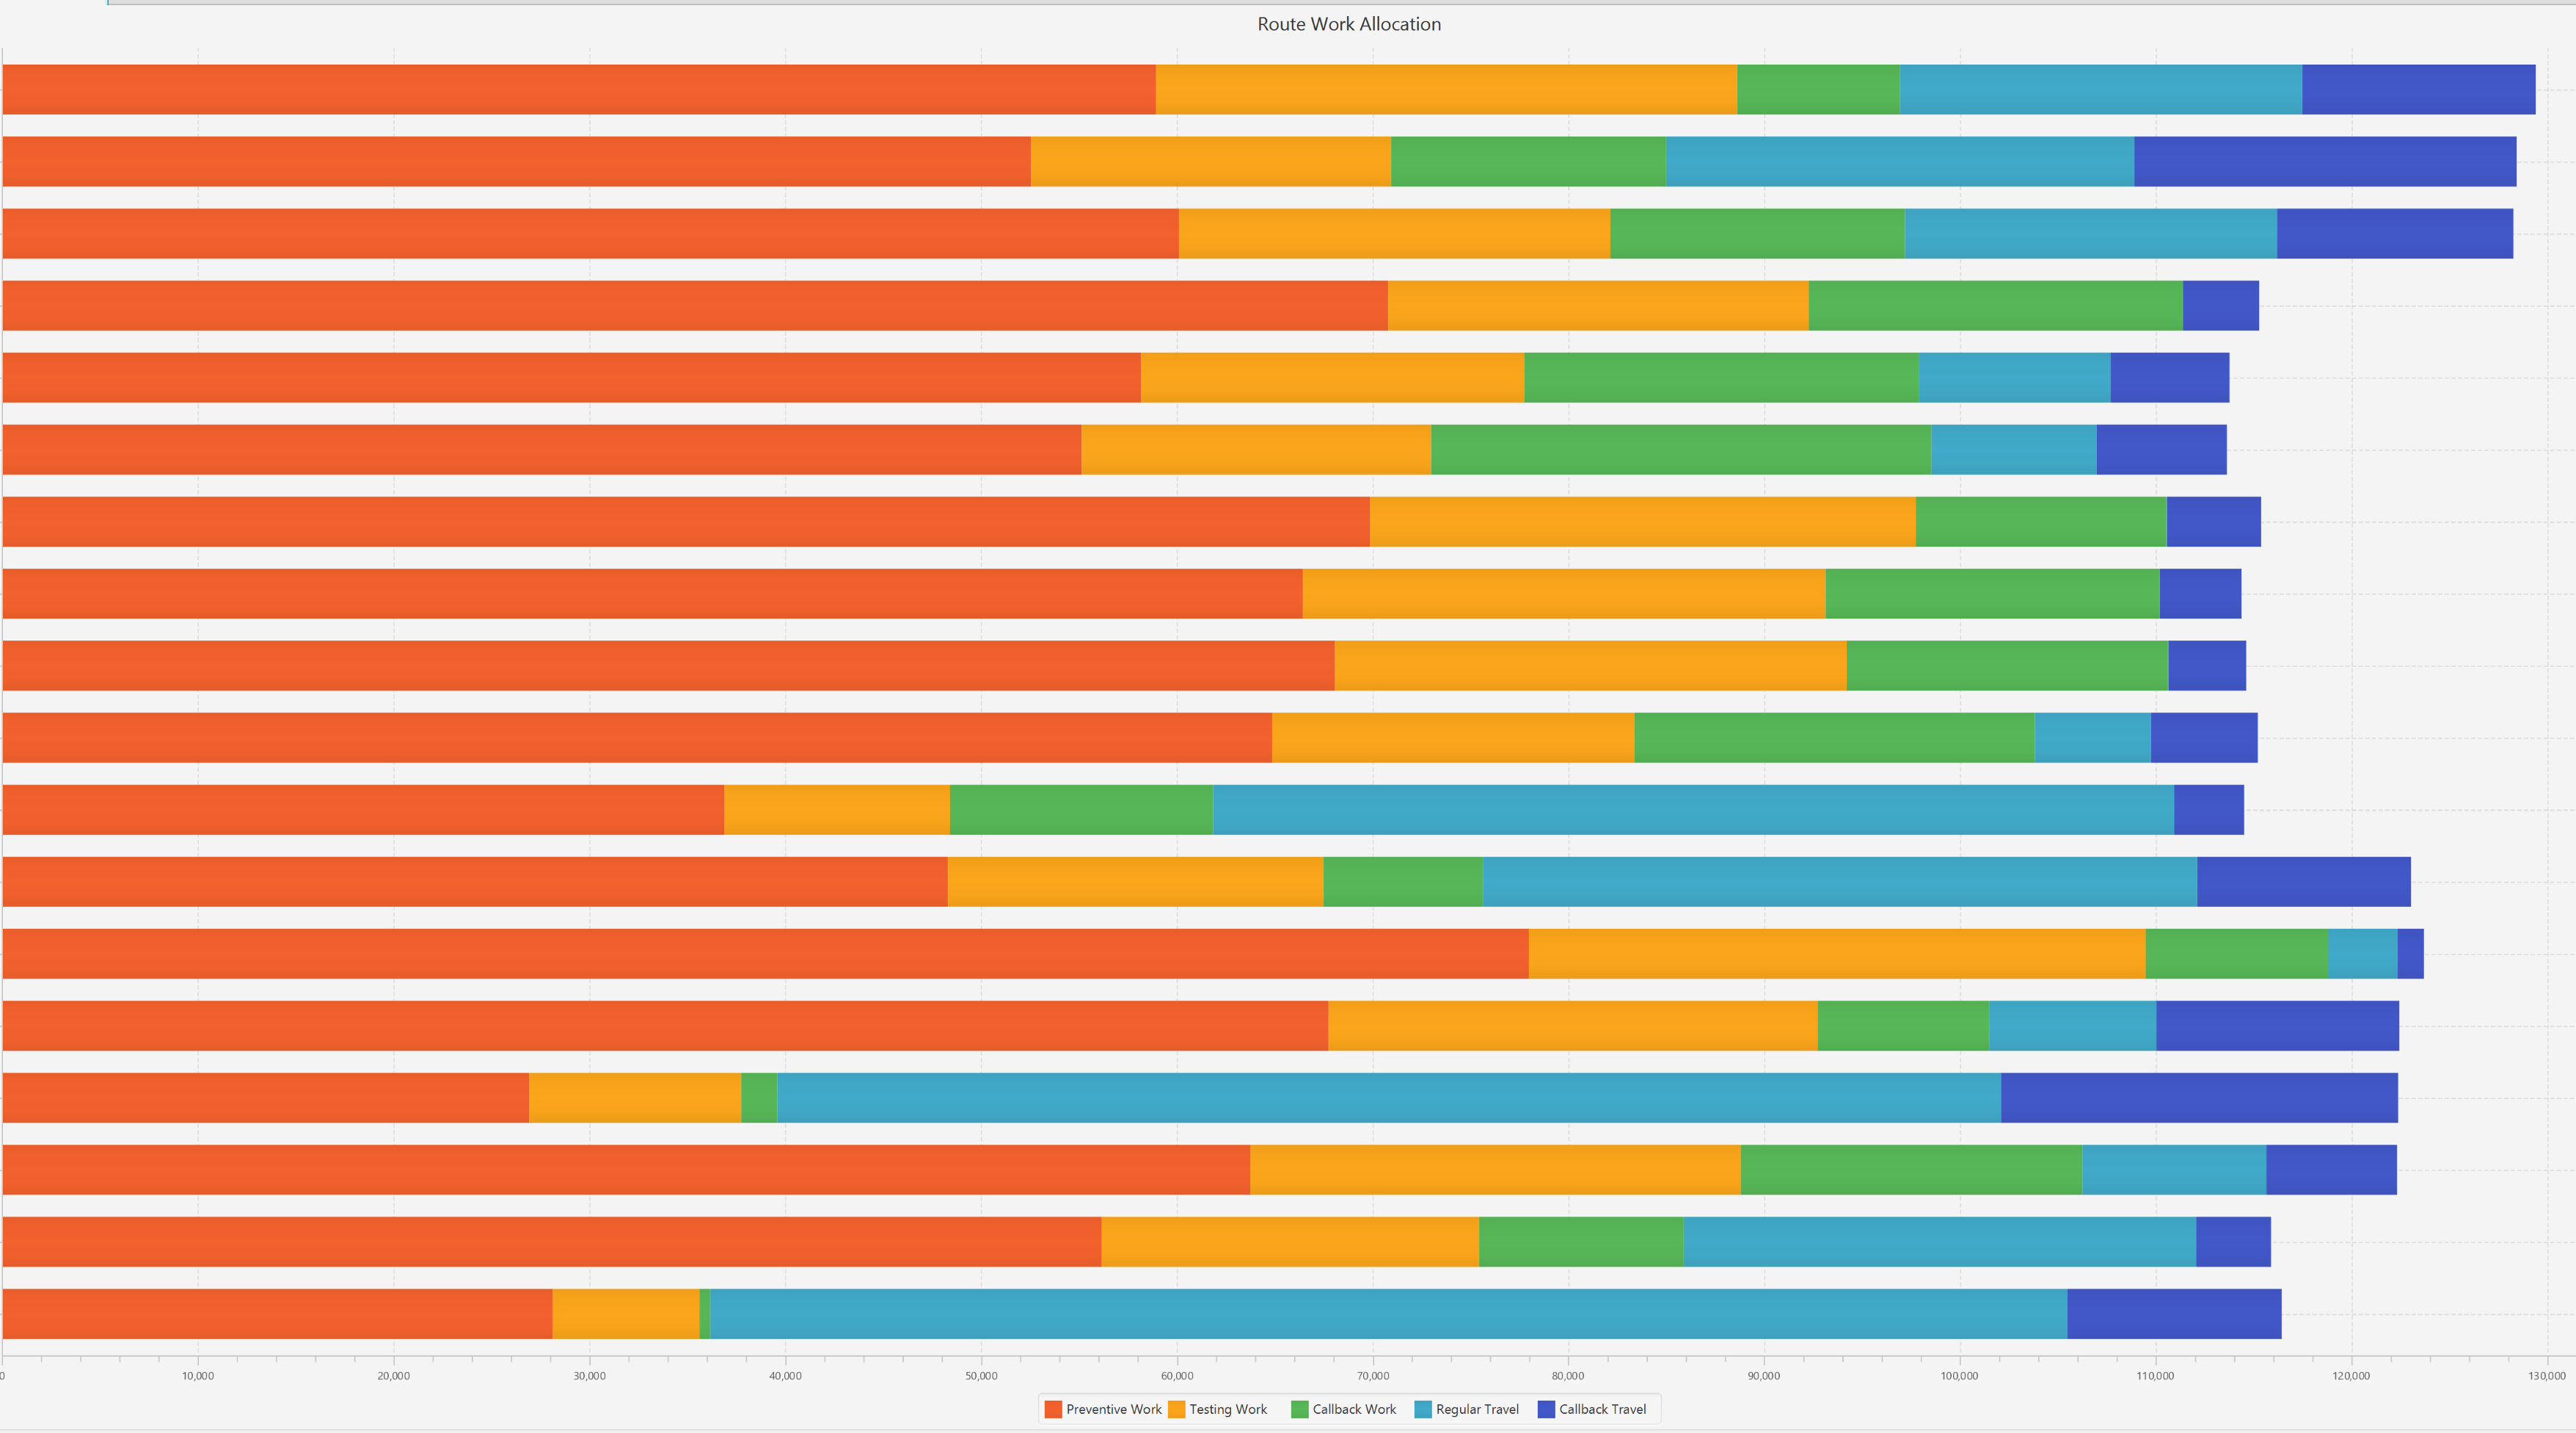
\includegraphics[width=11cm]{imagesfieldservice/barchartbalanced}
% \end{frame}

\begin{frame}
\frametitle{Scheduling: One Day of Monthly Plan}
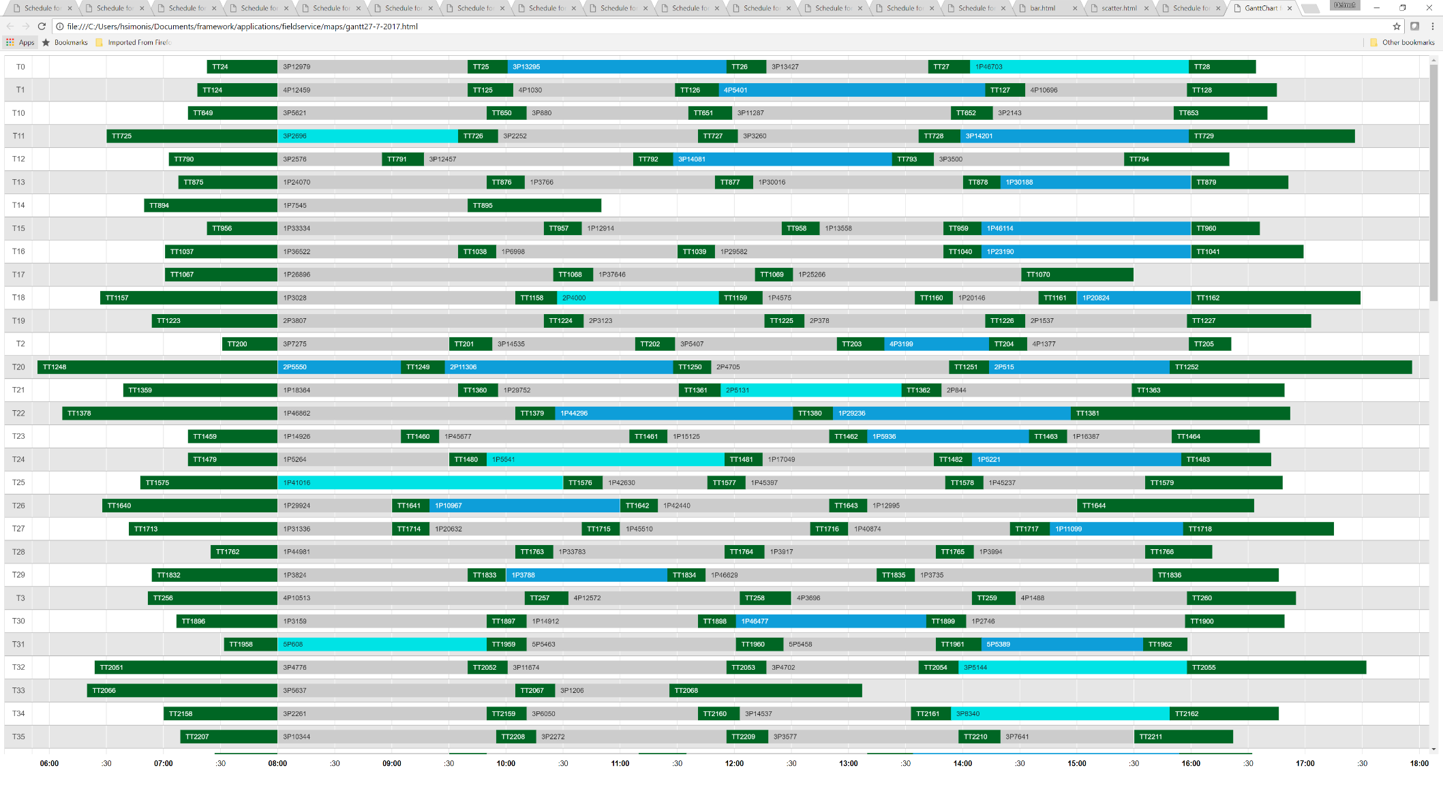
\includegraphics[width=11cm]{imagesfieldservice/schedule}
\end{frame}

\begin{frame}
\frametitle{Methods Used}
\begin{description}
\item[Clustering] Connected components on generated graph
\item[Routing] Which places to visit in one trip
\begin{itemize}
\item Core MIP Model
\item Iterative MIP inside Clustering
\item Two stage grouping of locations to reduce expected travel
\item Local Search
\end{itemize}
\item[Scheduling] Dynamic Programming and Set Partitioning
\end{description}
\end{frame}

%% \begin{frame}
%% \frametitle{Integration with Simulator, First Day}
%% 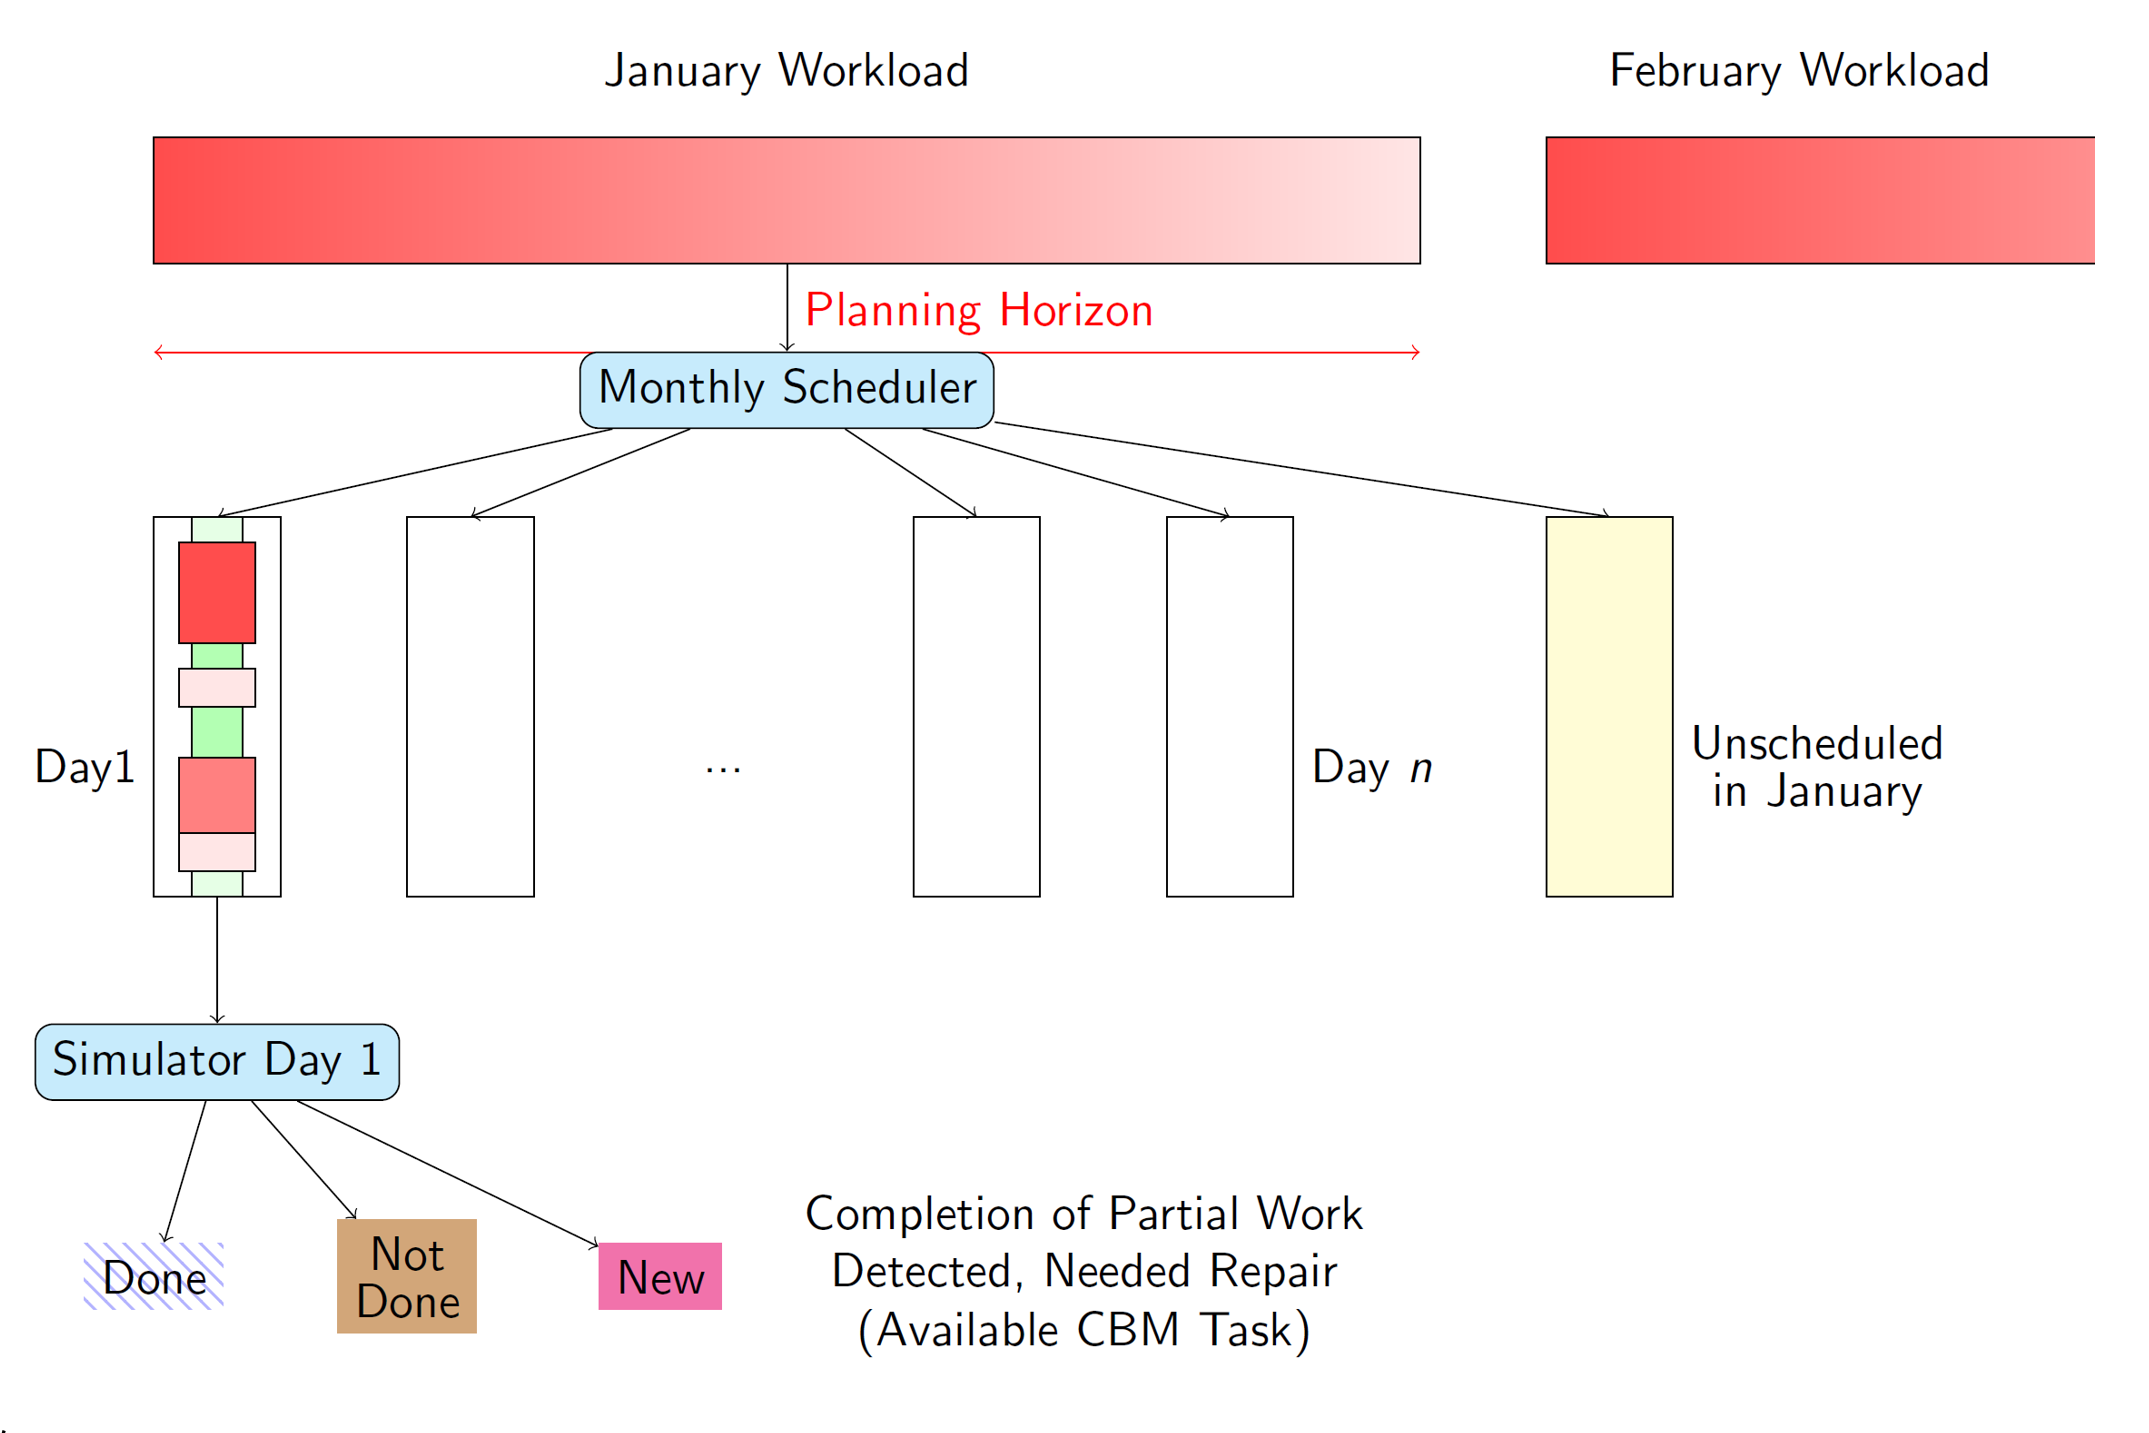
\includegraphics[width=11cm]{imagesfieldservice/integration1}
%% \end{frame}

%% \begin{frame}
%% \frametitle{Integration with Simulator, Next Day}
%% 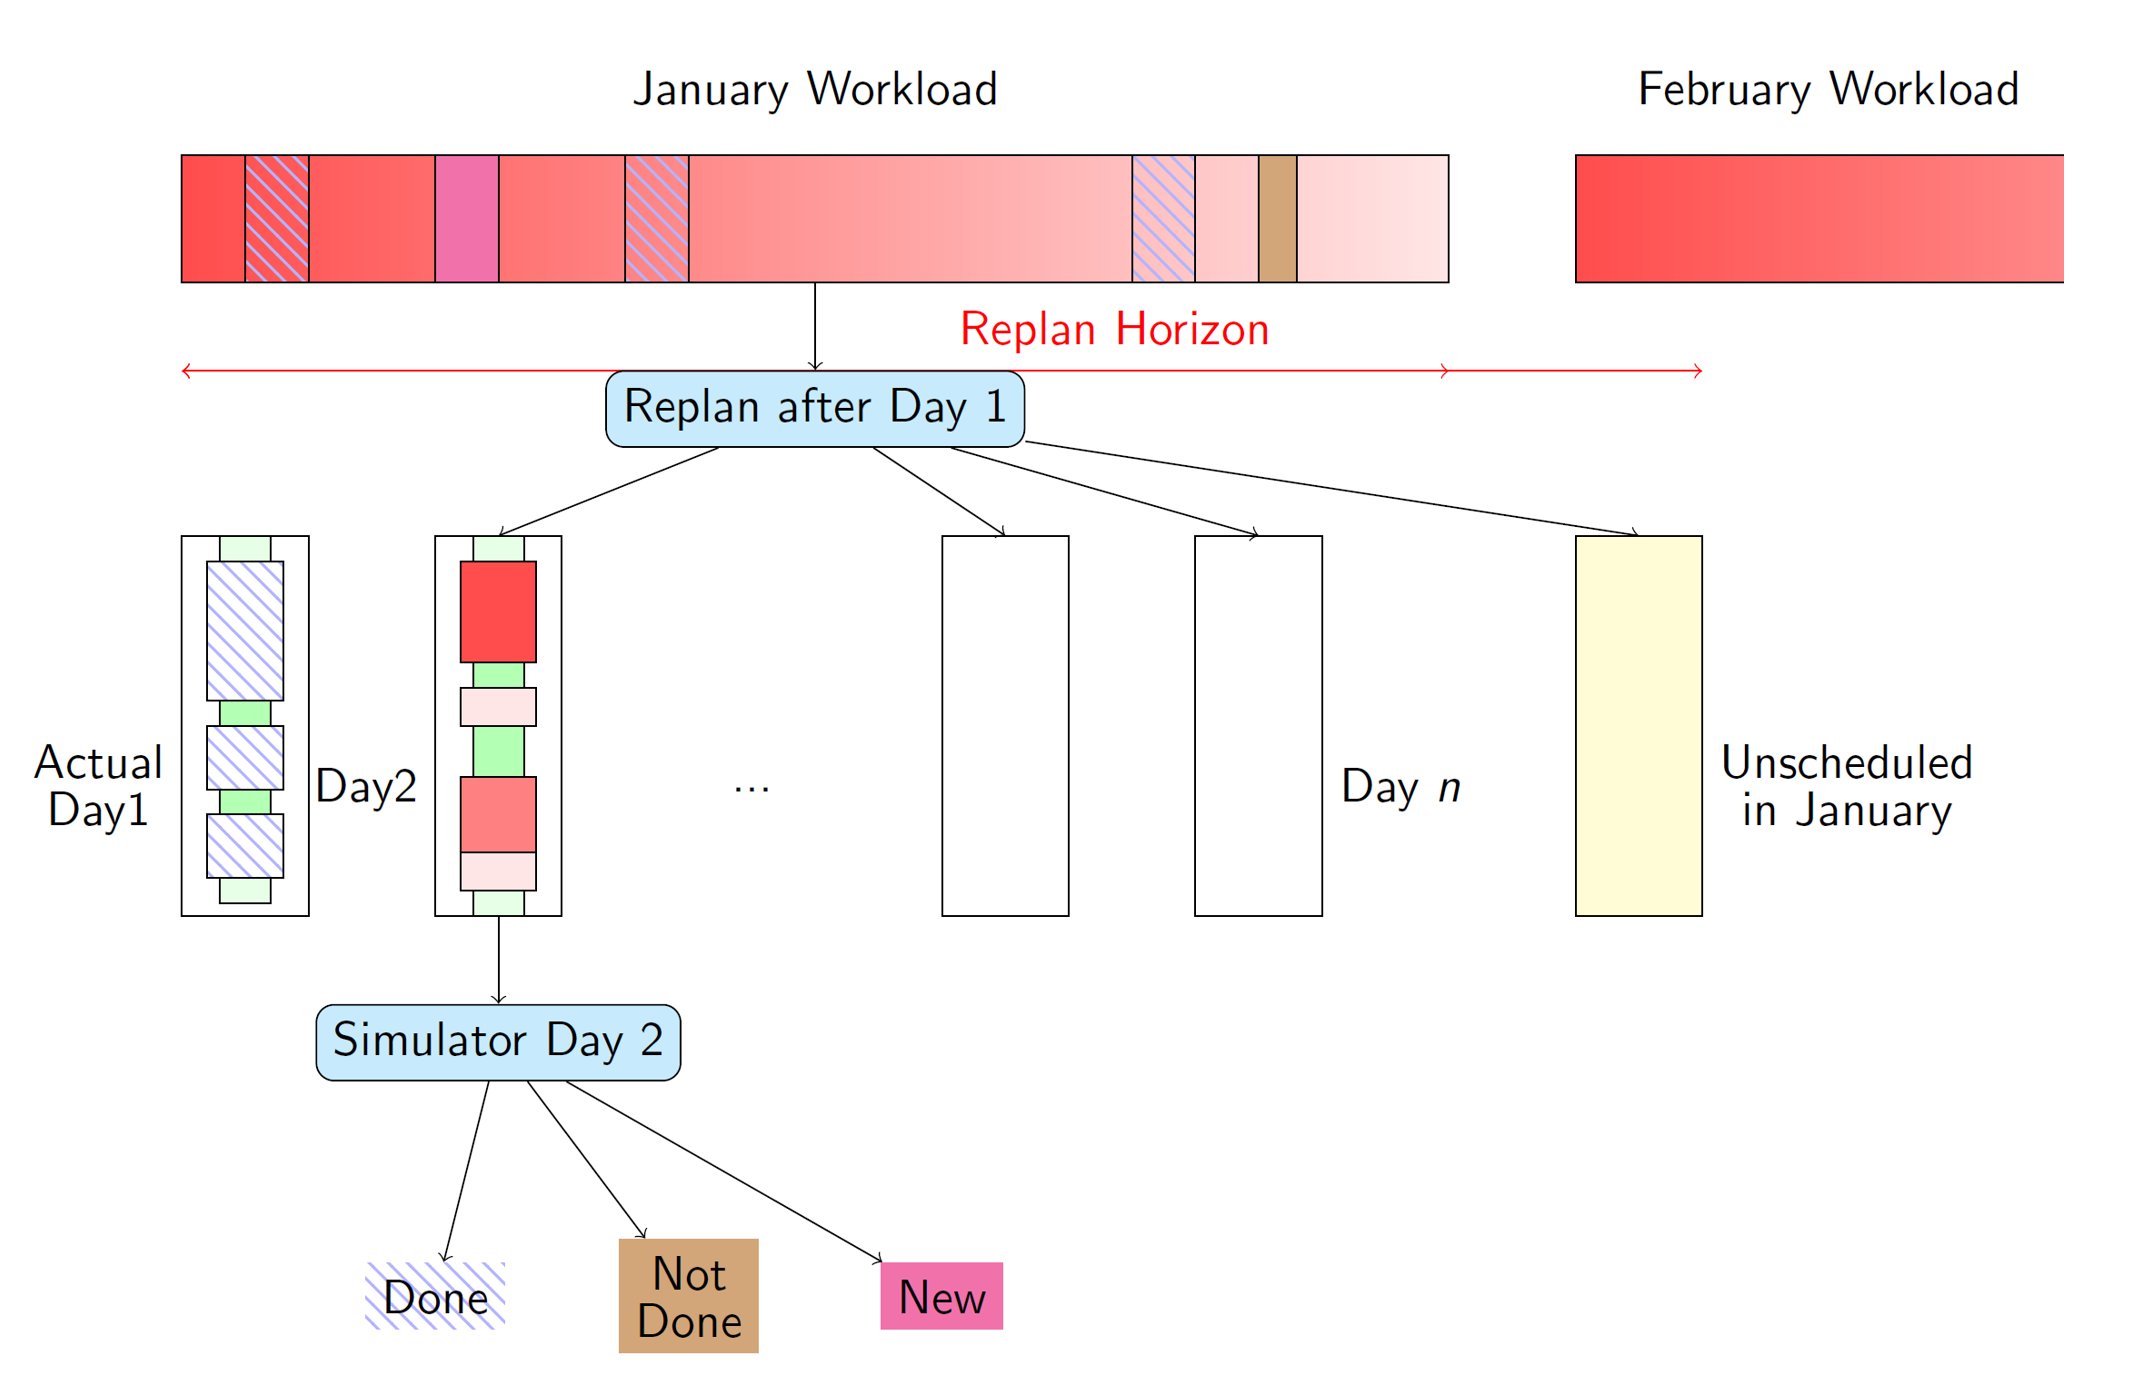
\includegraphics[width=11cm]{imagesfieldservice/integration2}
%% \end{frame}

% \begin{frame}
% \frametitle{Integration with Simulator, First Day}
% 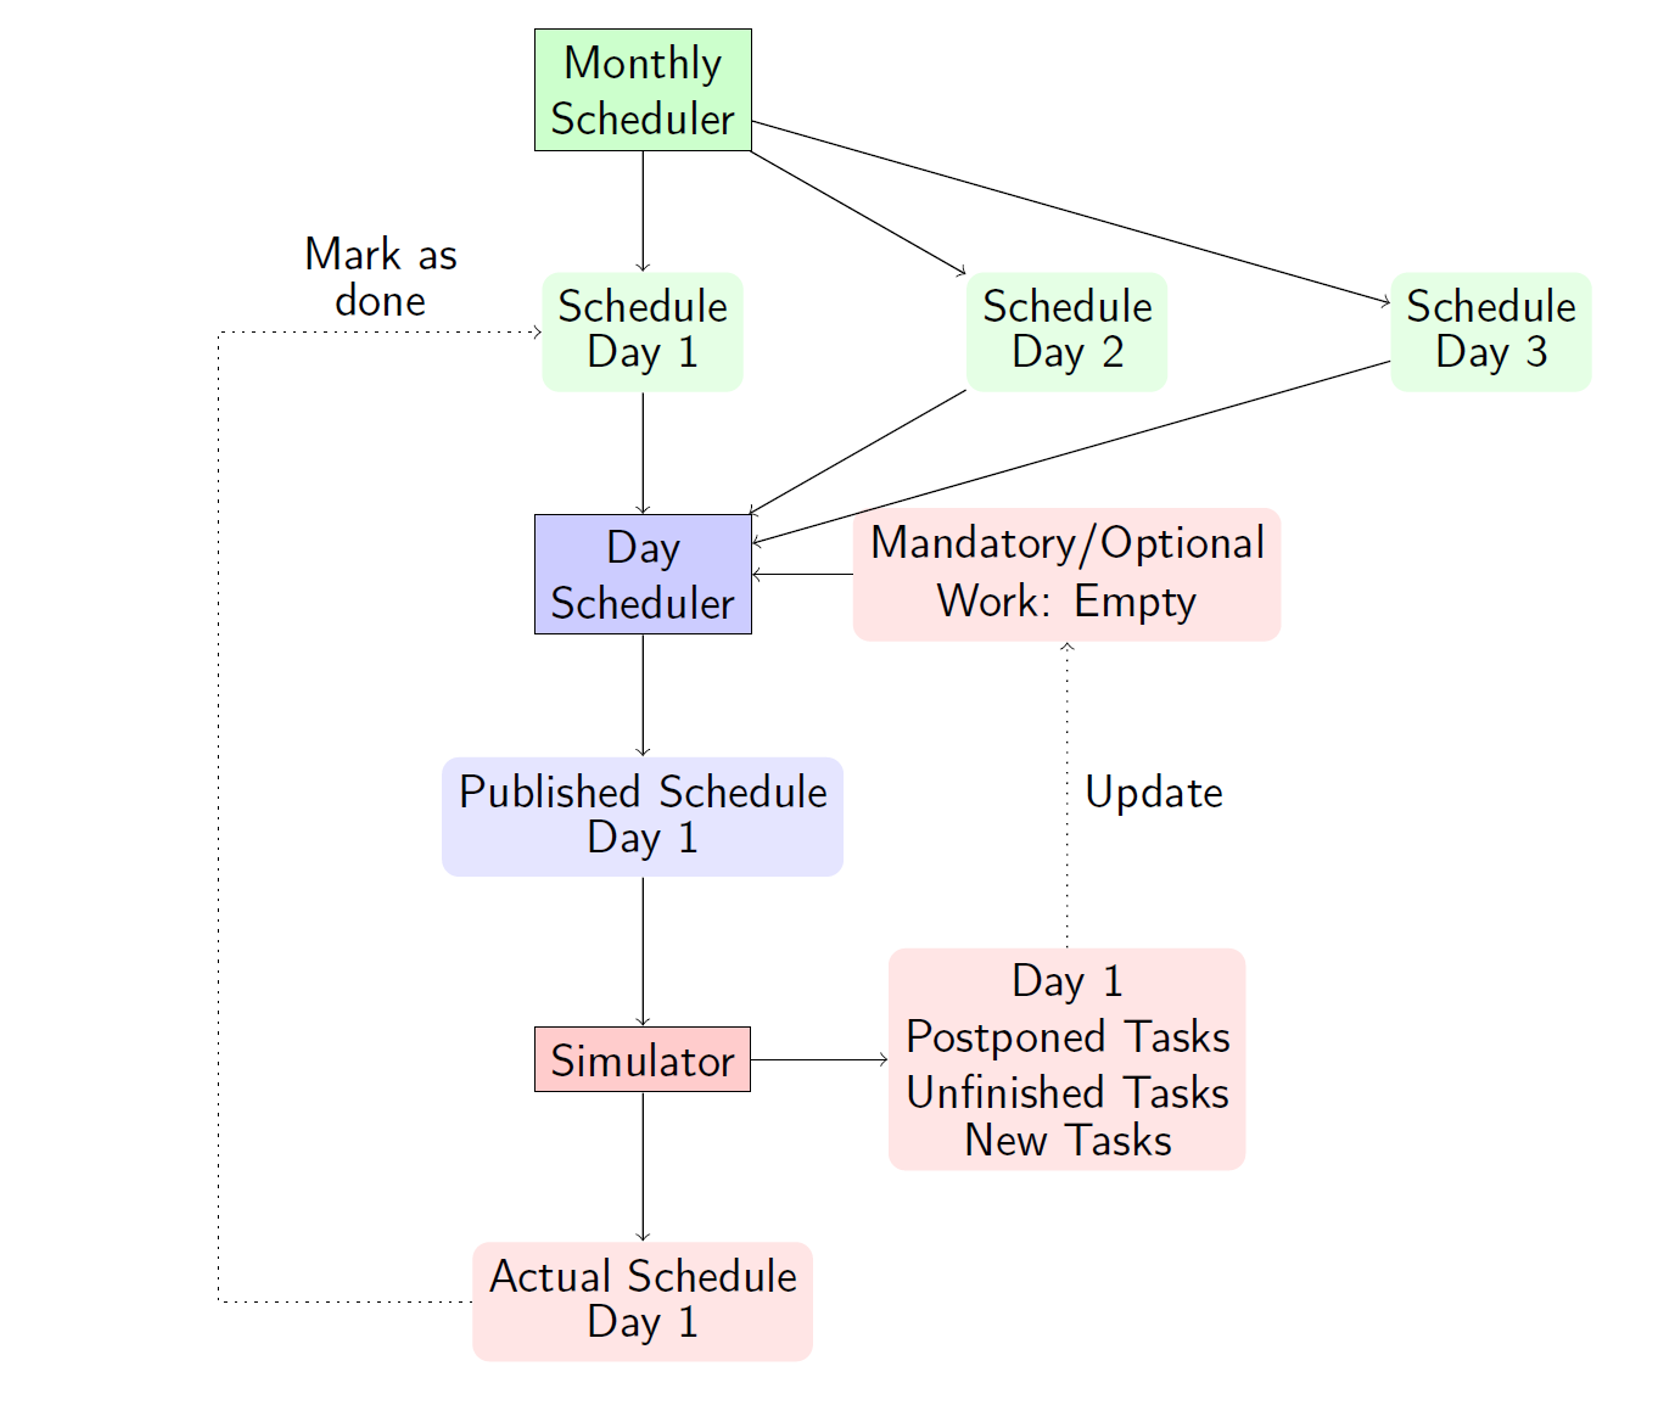
\includegraphics[width=8cm]{imagesfieldservice/dayscheduler1}
% \end{frame}

% \begin{frame}
% \frametitle{Integration with Simulator, Next Day}
% 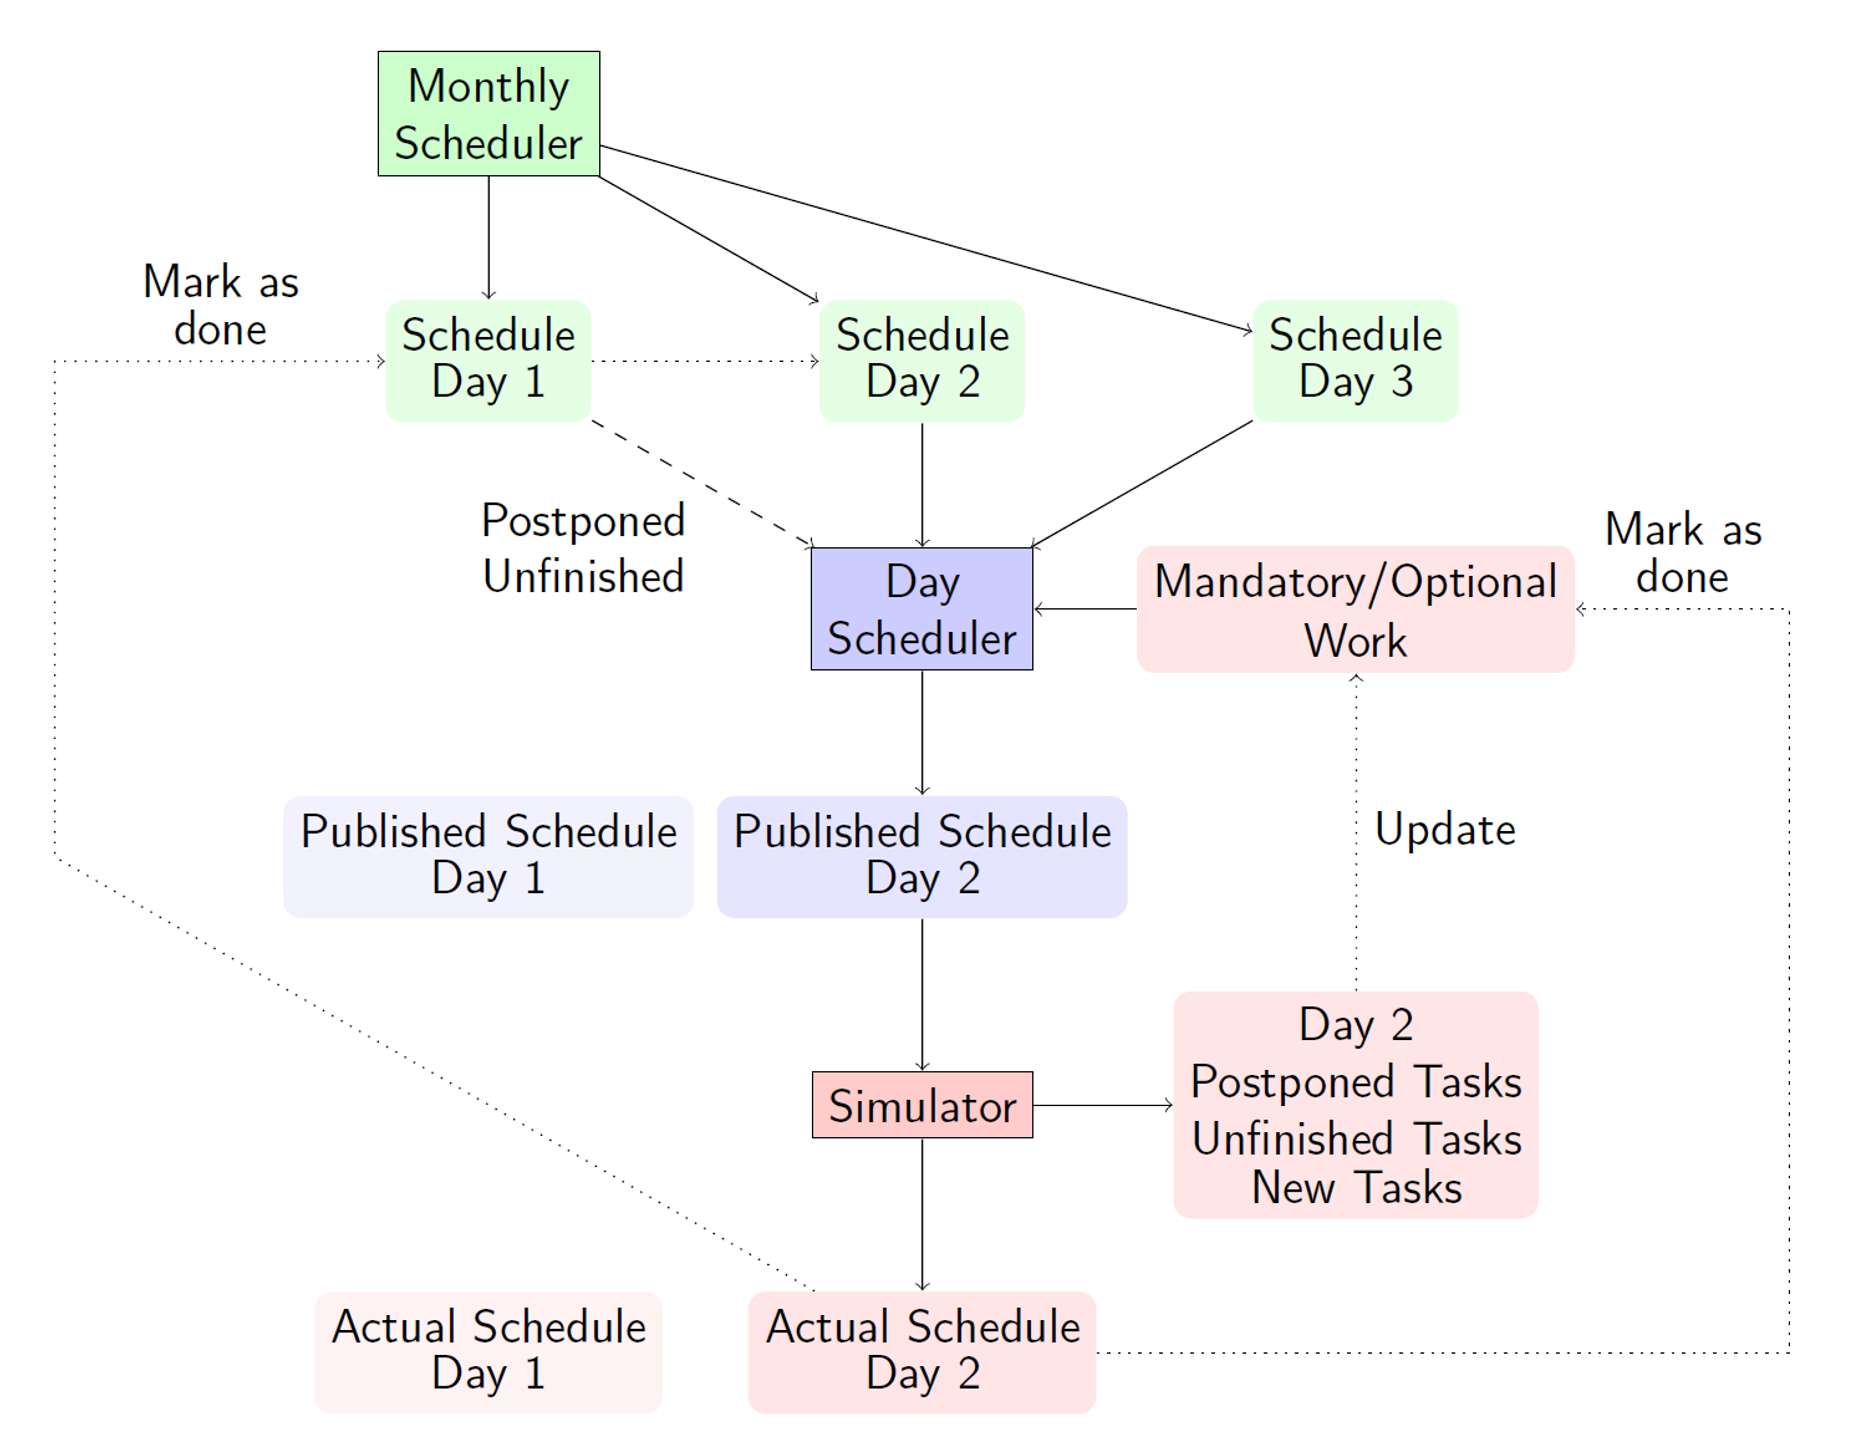
\includegraphics[width=8cm]{imagesfieldservice/dayscheduler2}
% \end{frame}

\begin{frame}
\frametitle{Simulator Process Modelling}
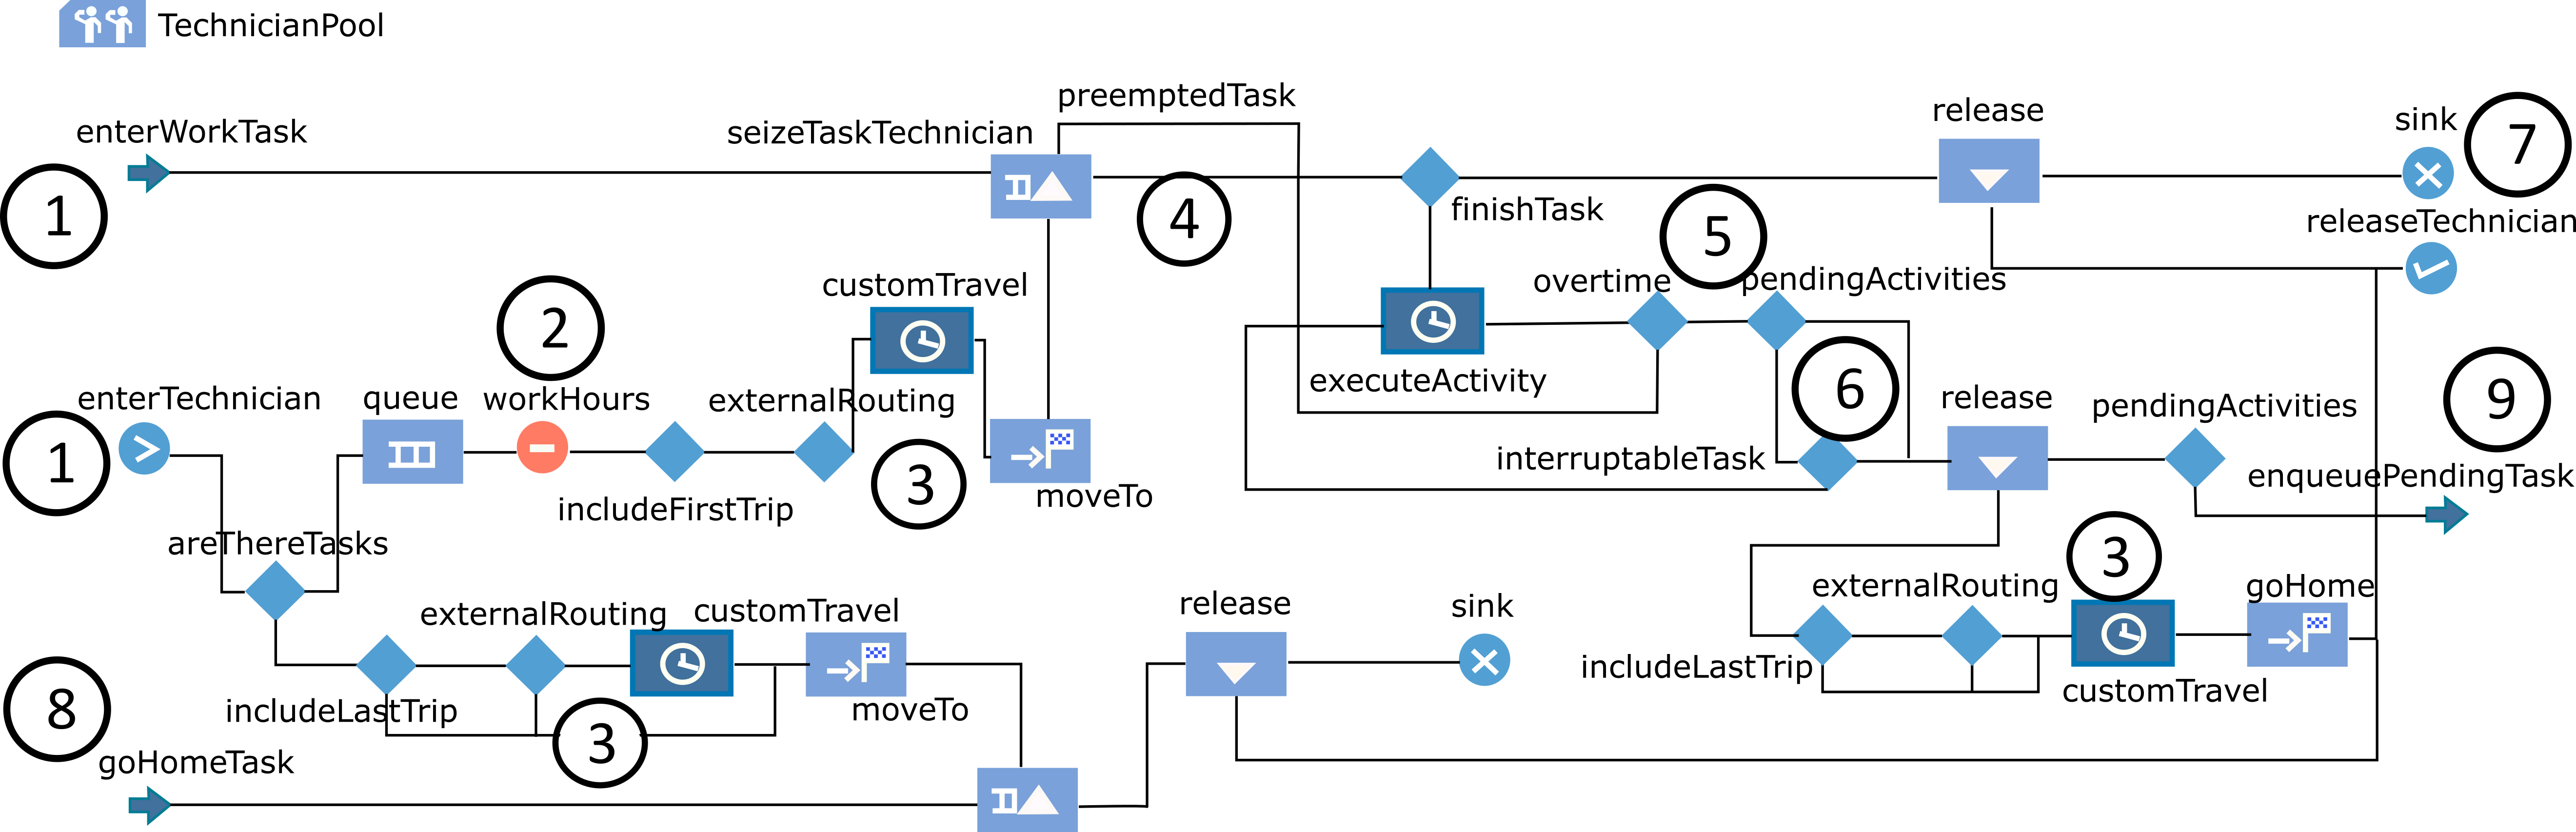
\includegraphics[width=11cm]{imagesfieldservice/processmodelling}
\end{frame}

\begin{frame}
\frametitle{Dealing with Unplanned Callbacks}
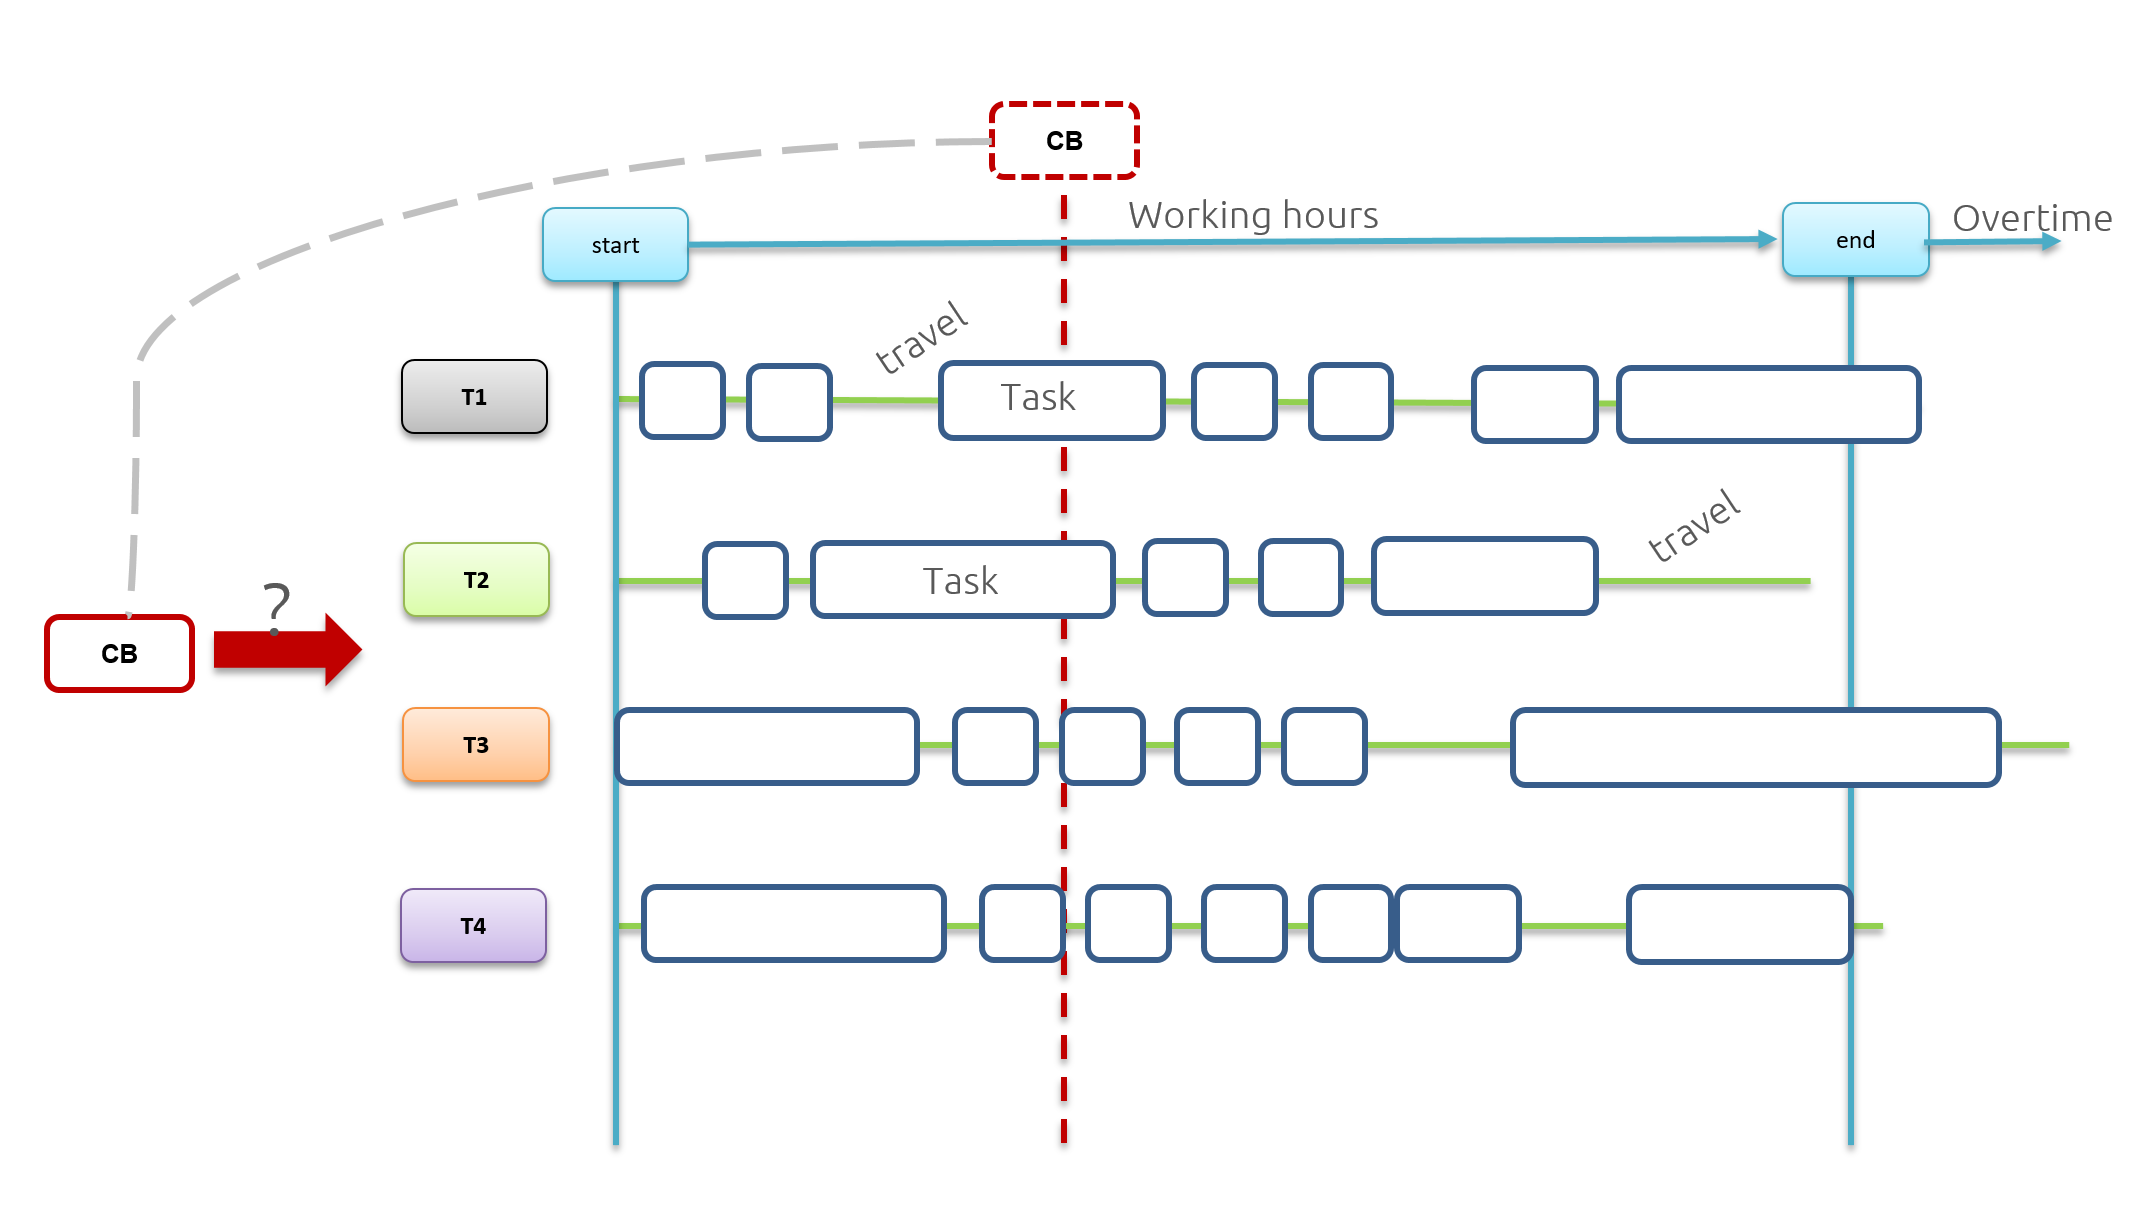
\includegraphics[width=10cm]{imagesfieldservice/callbacks}
\begin{itemize}
\item Who is dealing with the callback?
\item How to adjust the schedule after callback?
\end{itemize}
\end{frame}

\subsection{Evaluation}

\begin{frame}
\frametitle{Use Cases}
\begin{itemize}
\item Compare variants of problem to understand impact of changes
\item Examples
\begin{itemize}
\item Where to place depots and their area? 
\item How many technicians are needed in which depots?
\item Should technicians do both planned and unplanned work?
\item When is overtime the better choice?
\end{itemize}
\end{itemize}
\end{frame}

\begin{frame}
\frametitle{Scenario Evaluation: KPI Comparison}
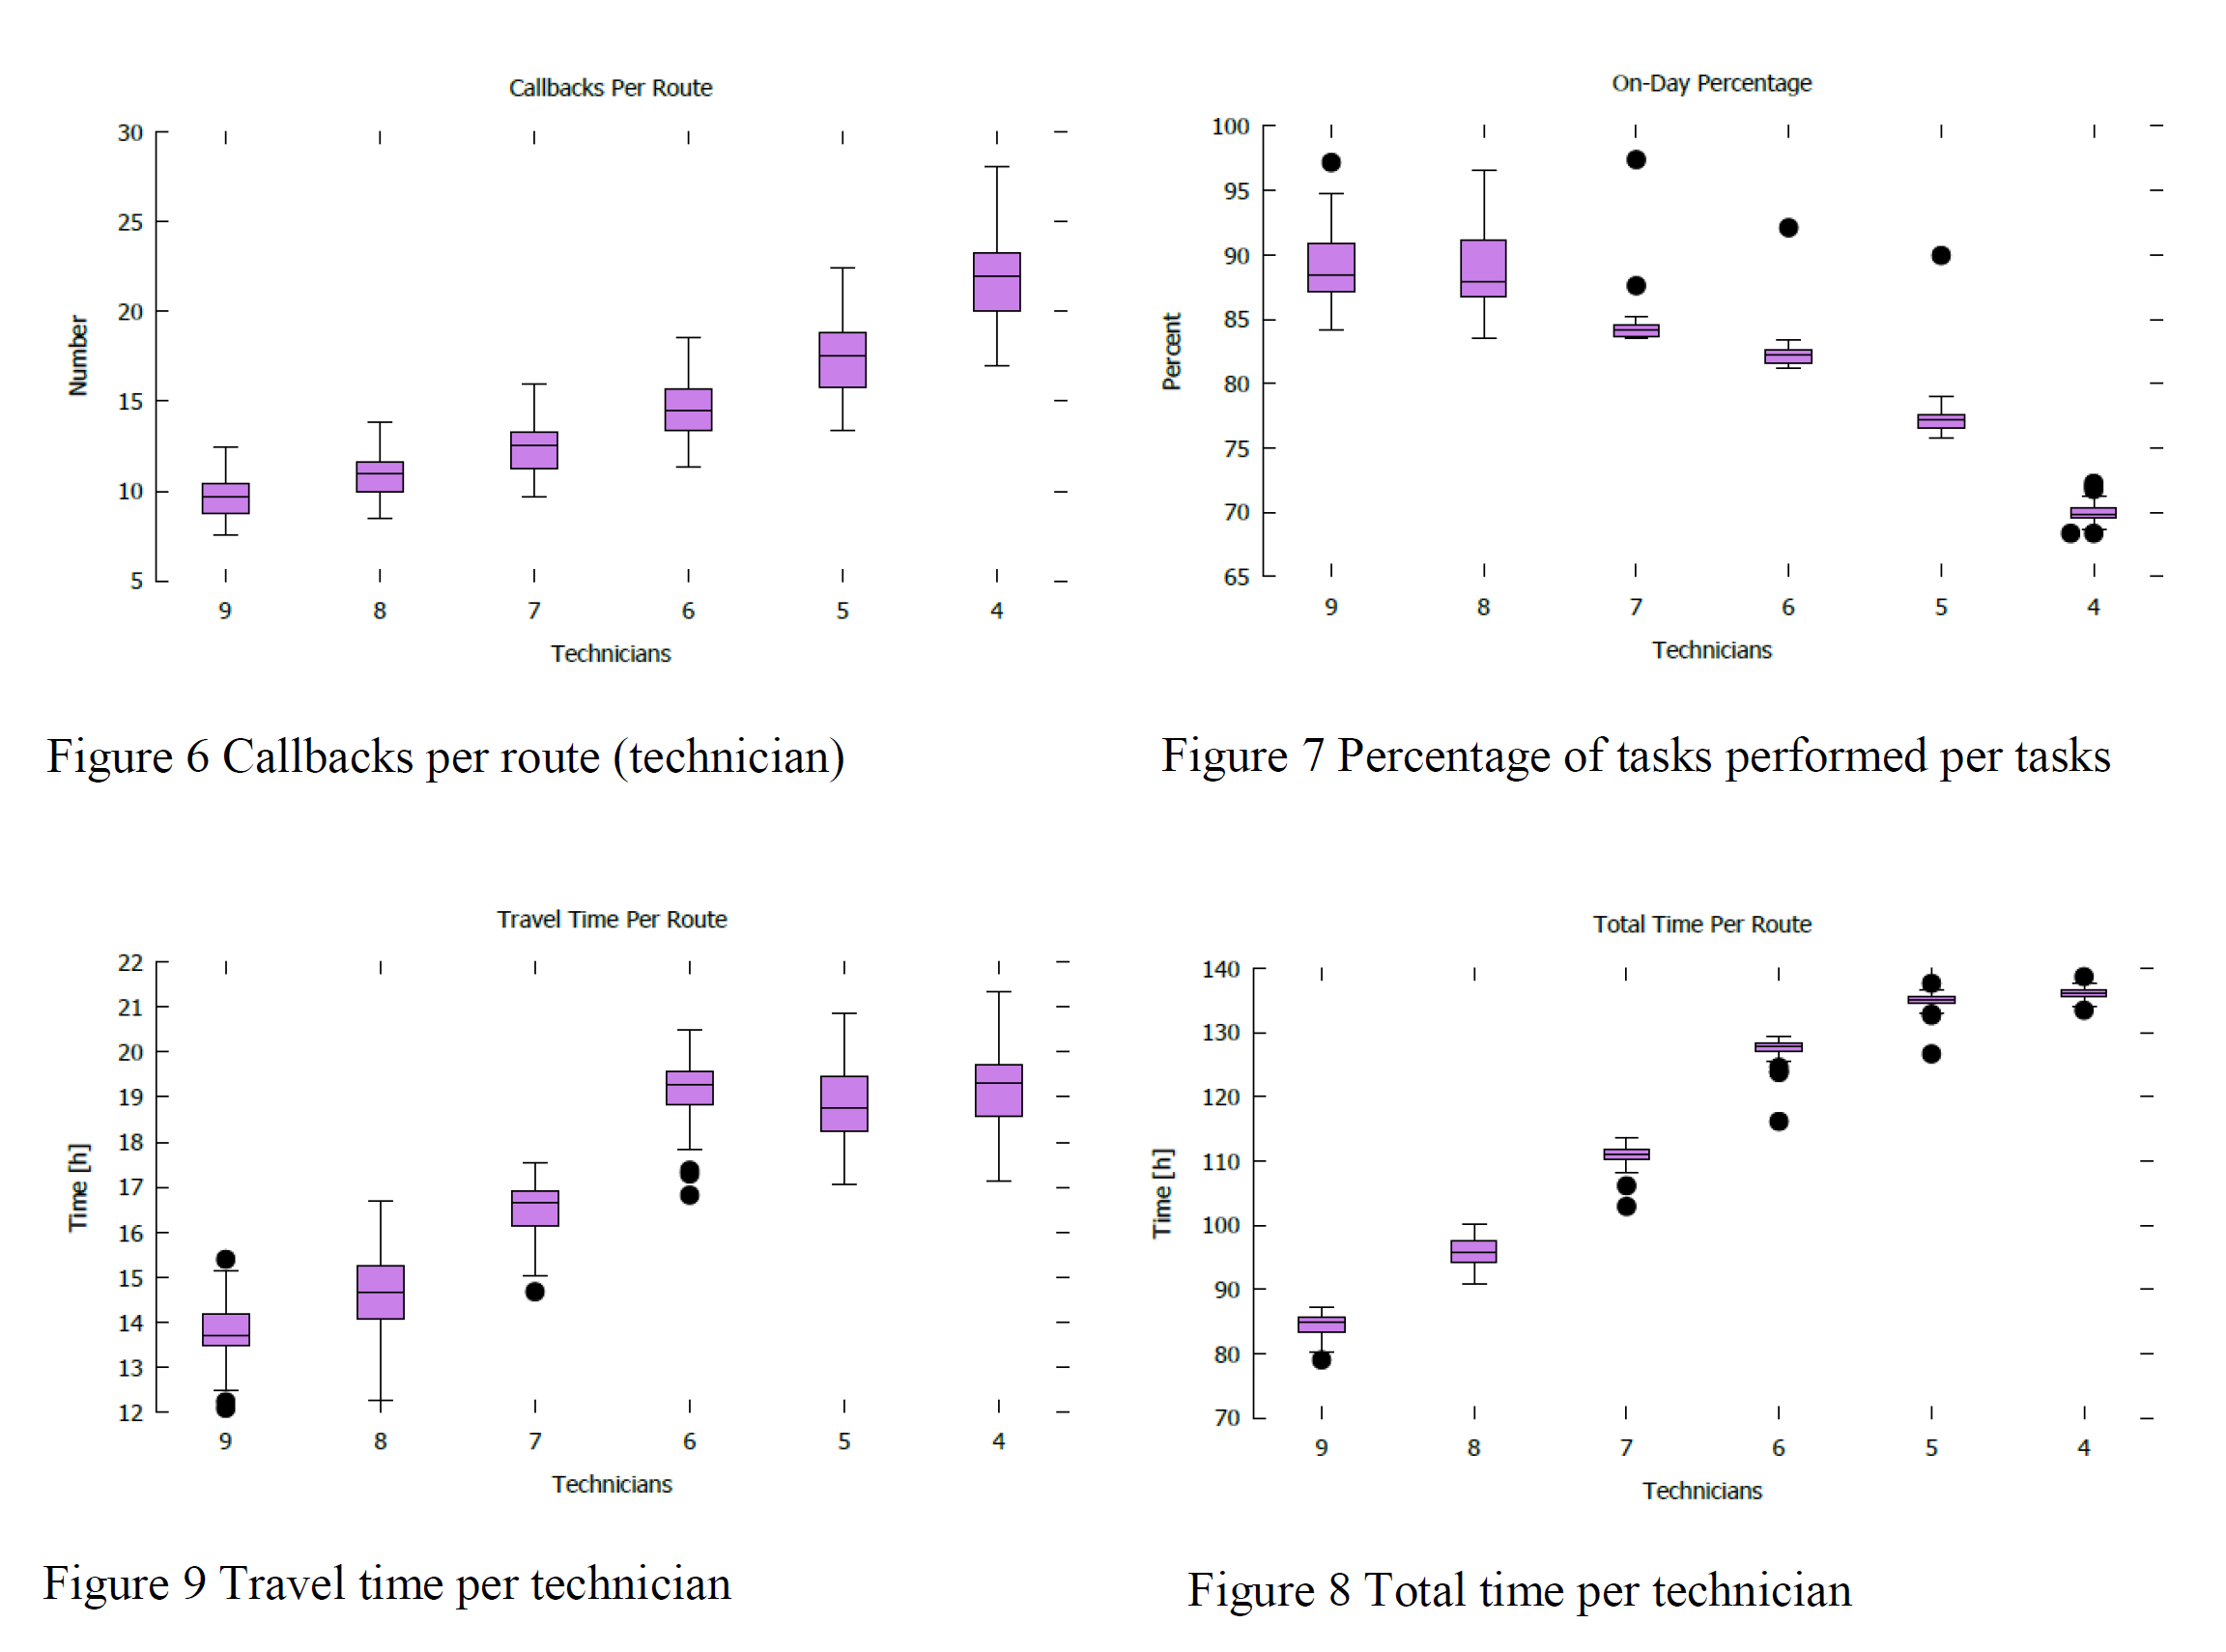
\includegraphics[width=9cm]{imagesfieldservice/scenarioevaluation}
\end{frame}

\begin{frame}
\frametitle{Scenario Evaluation: Qualitative Differences}
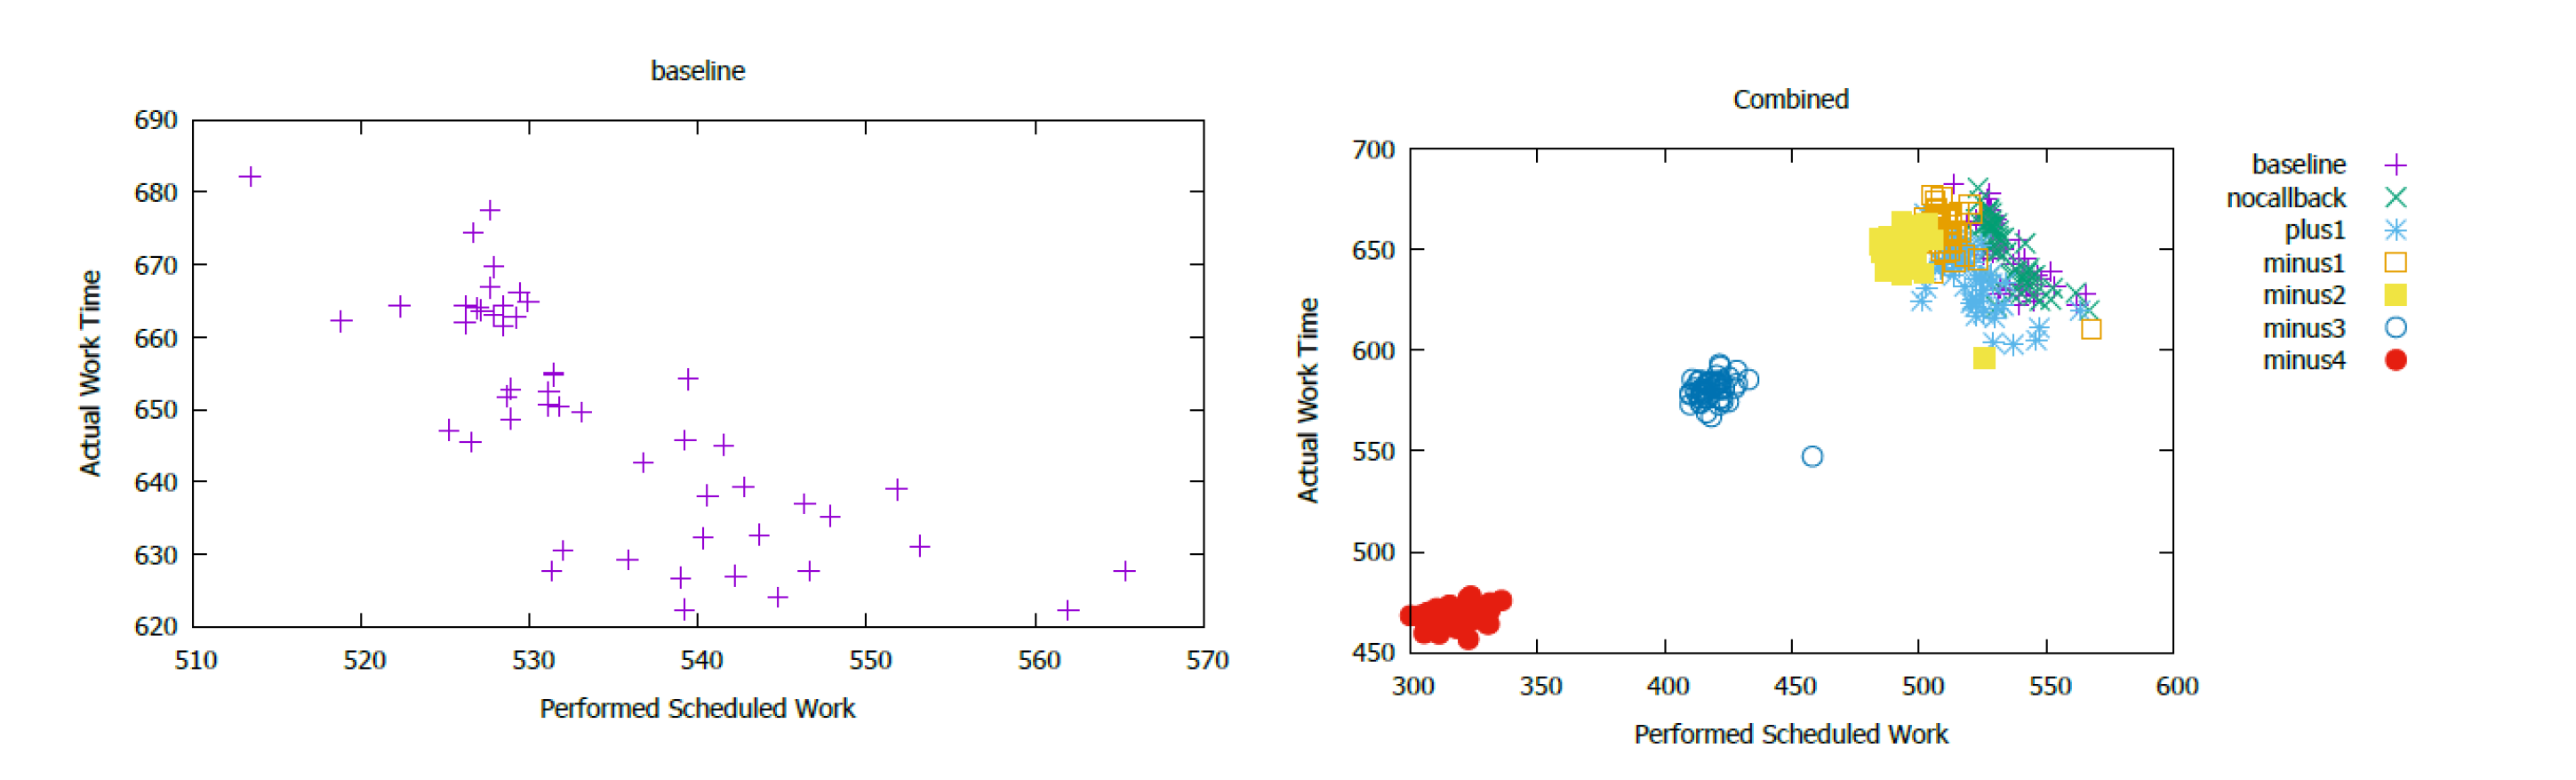
\includegraphics[width=10cm]{imagesfieldservice/scheduledactualwork}
\begin{itemize}
\item On left, each point shows the outcome of one month of optimization+simulation
\item On right, compare outcomes for different scenarios, clear clustering of results
\end{itemize}
\end{frame}

% \begin{frame}
% \frametitle{Scenario Evaluation: Drill-down to Details}
% 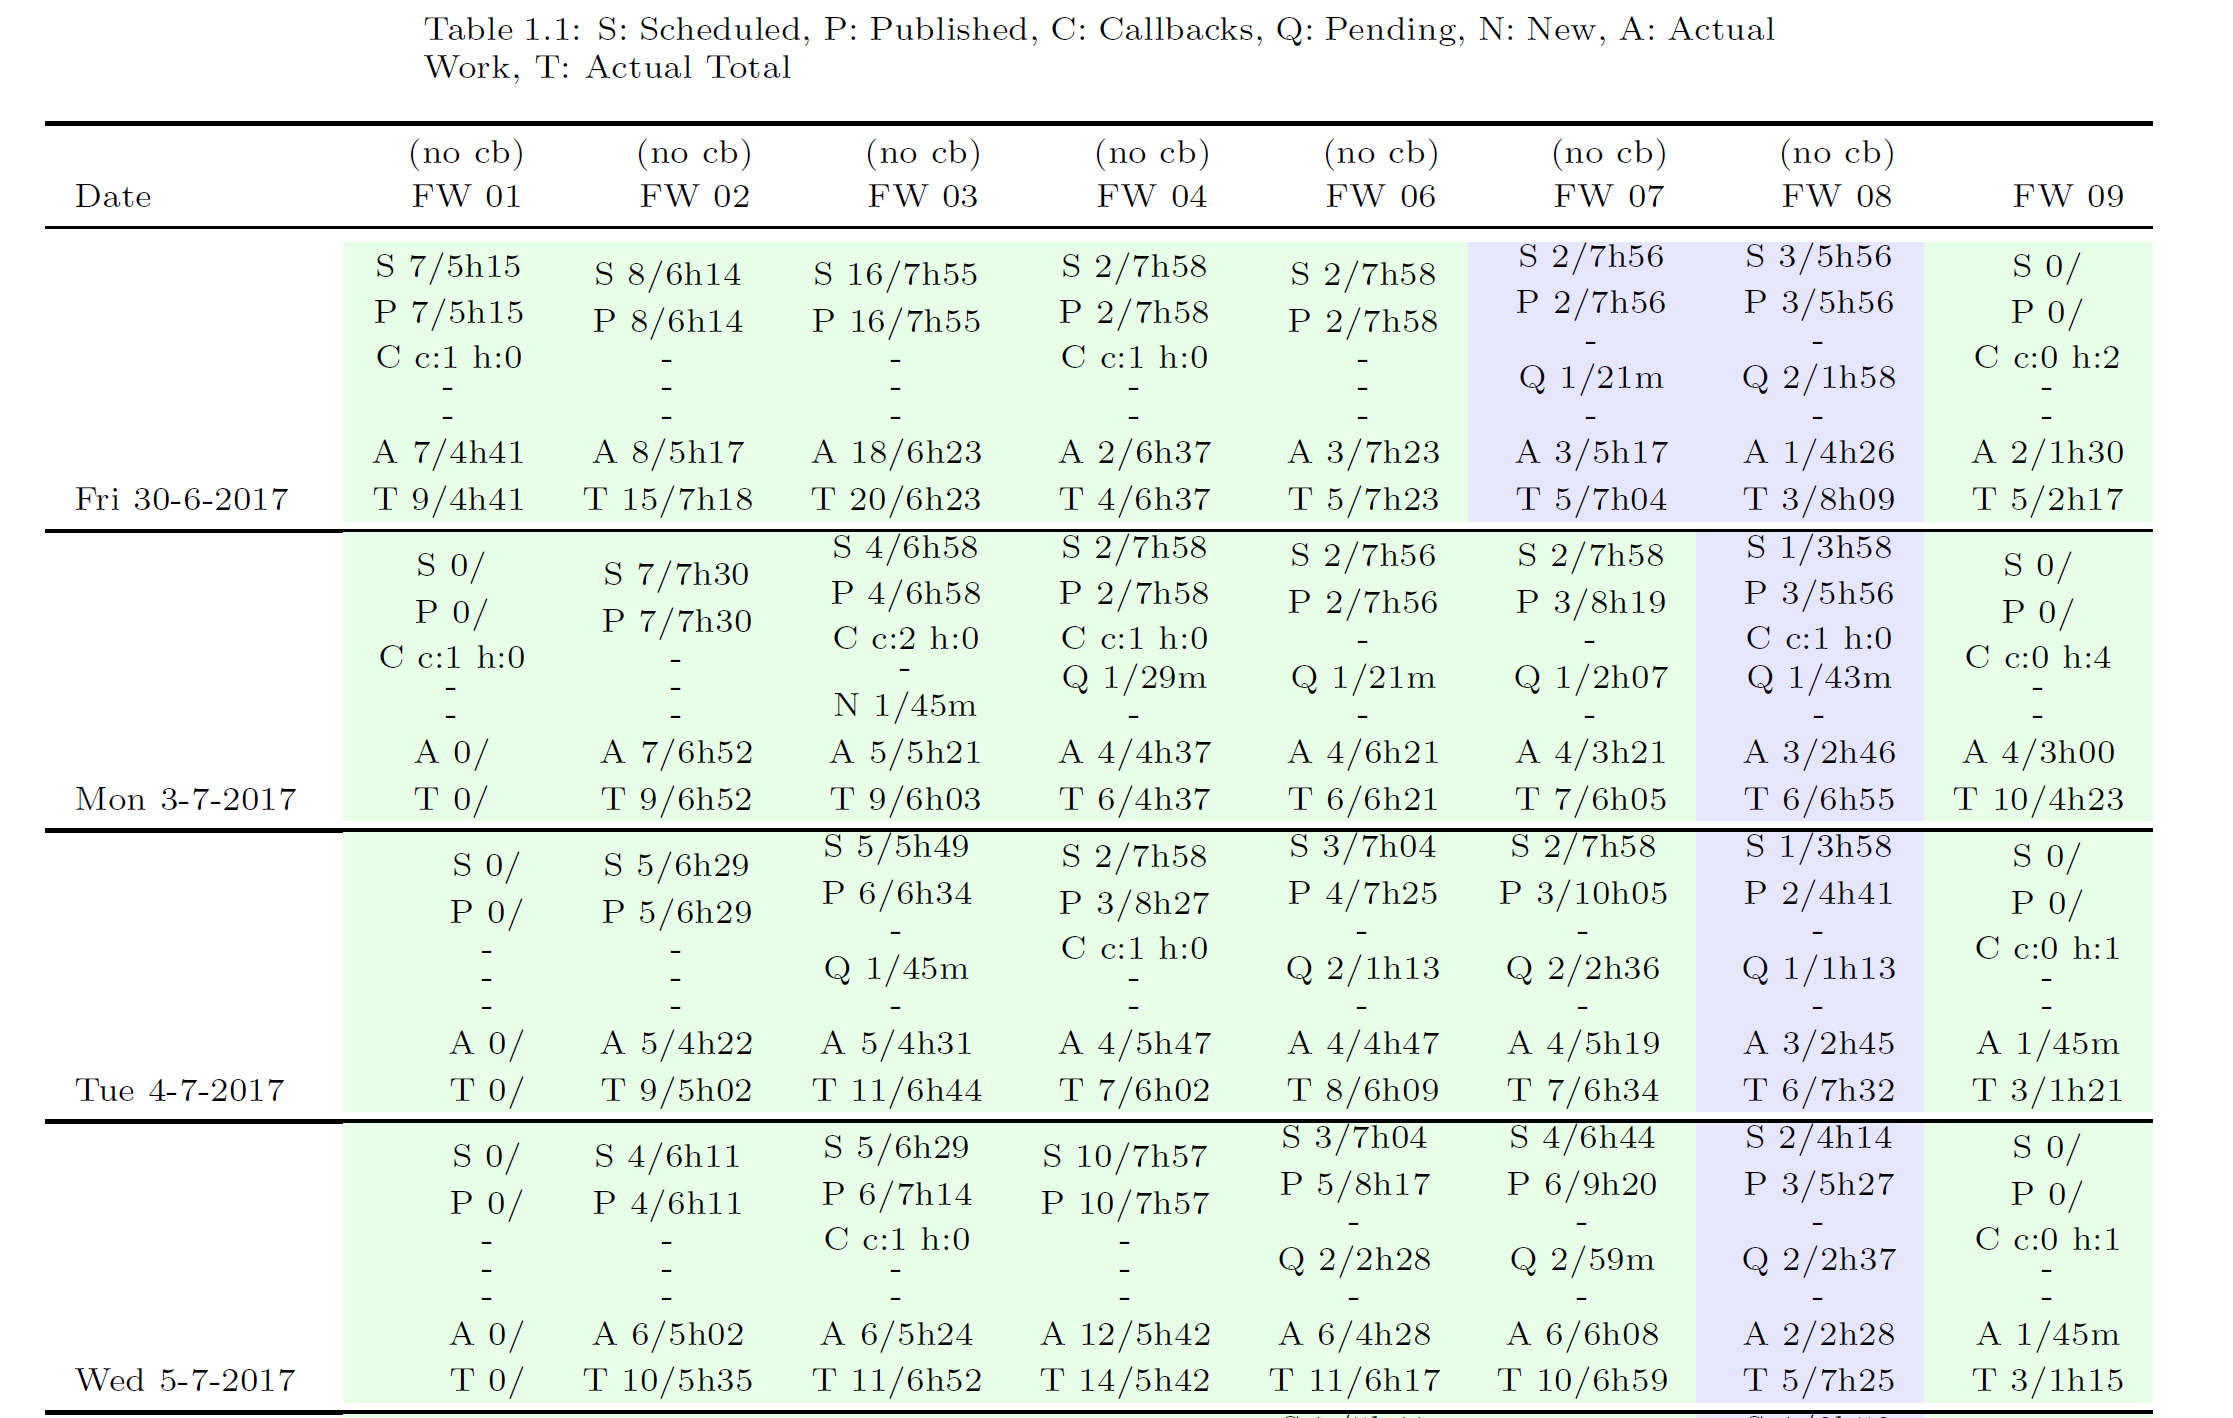
\includegraphics[width=11cm]{imagesfieldservice/detailsoverview}
% \end{frame}

% \begin{frame}
% \frametitle{Scenario Evaluation: Further Drill-down}
% 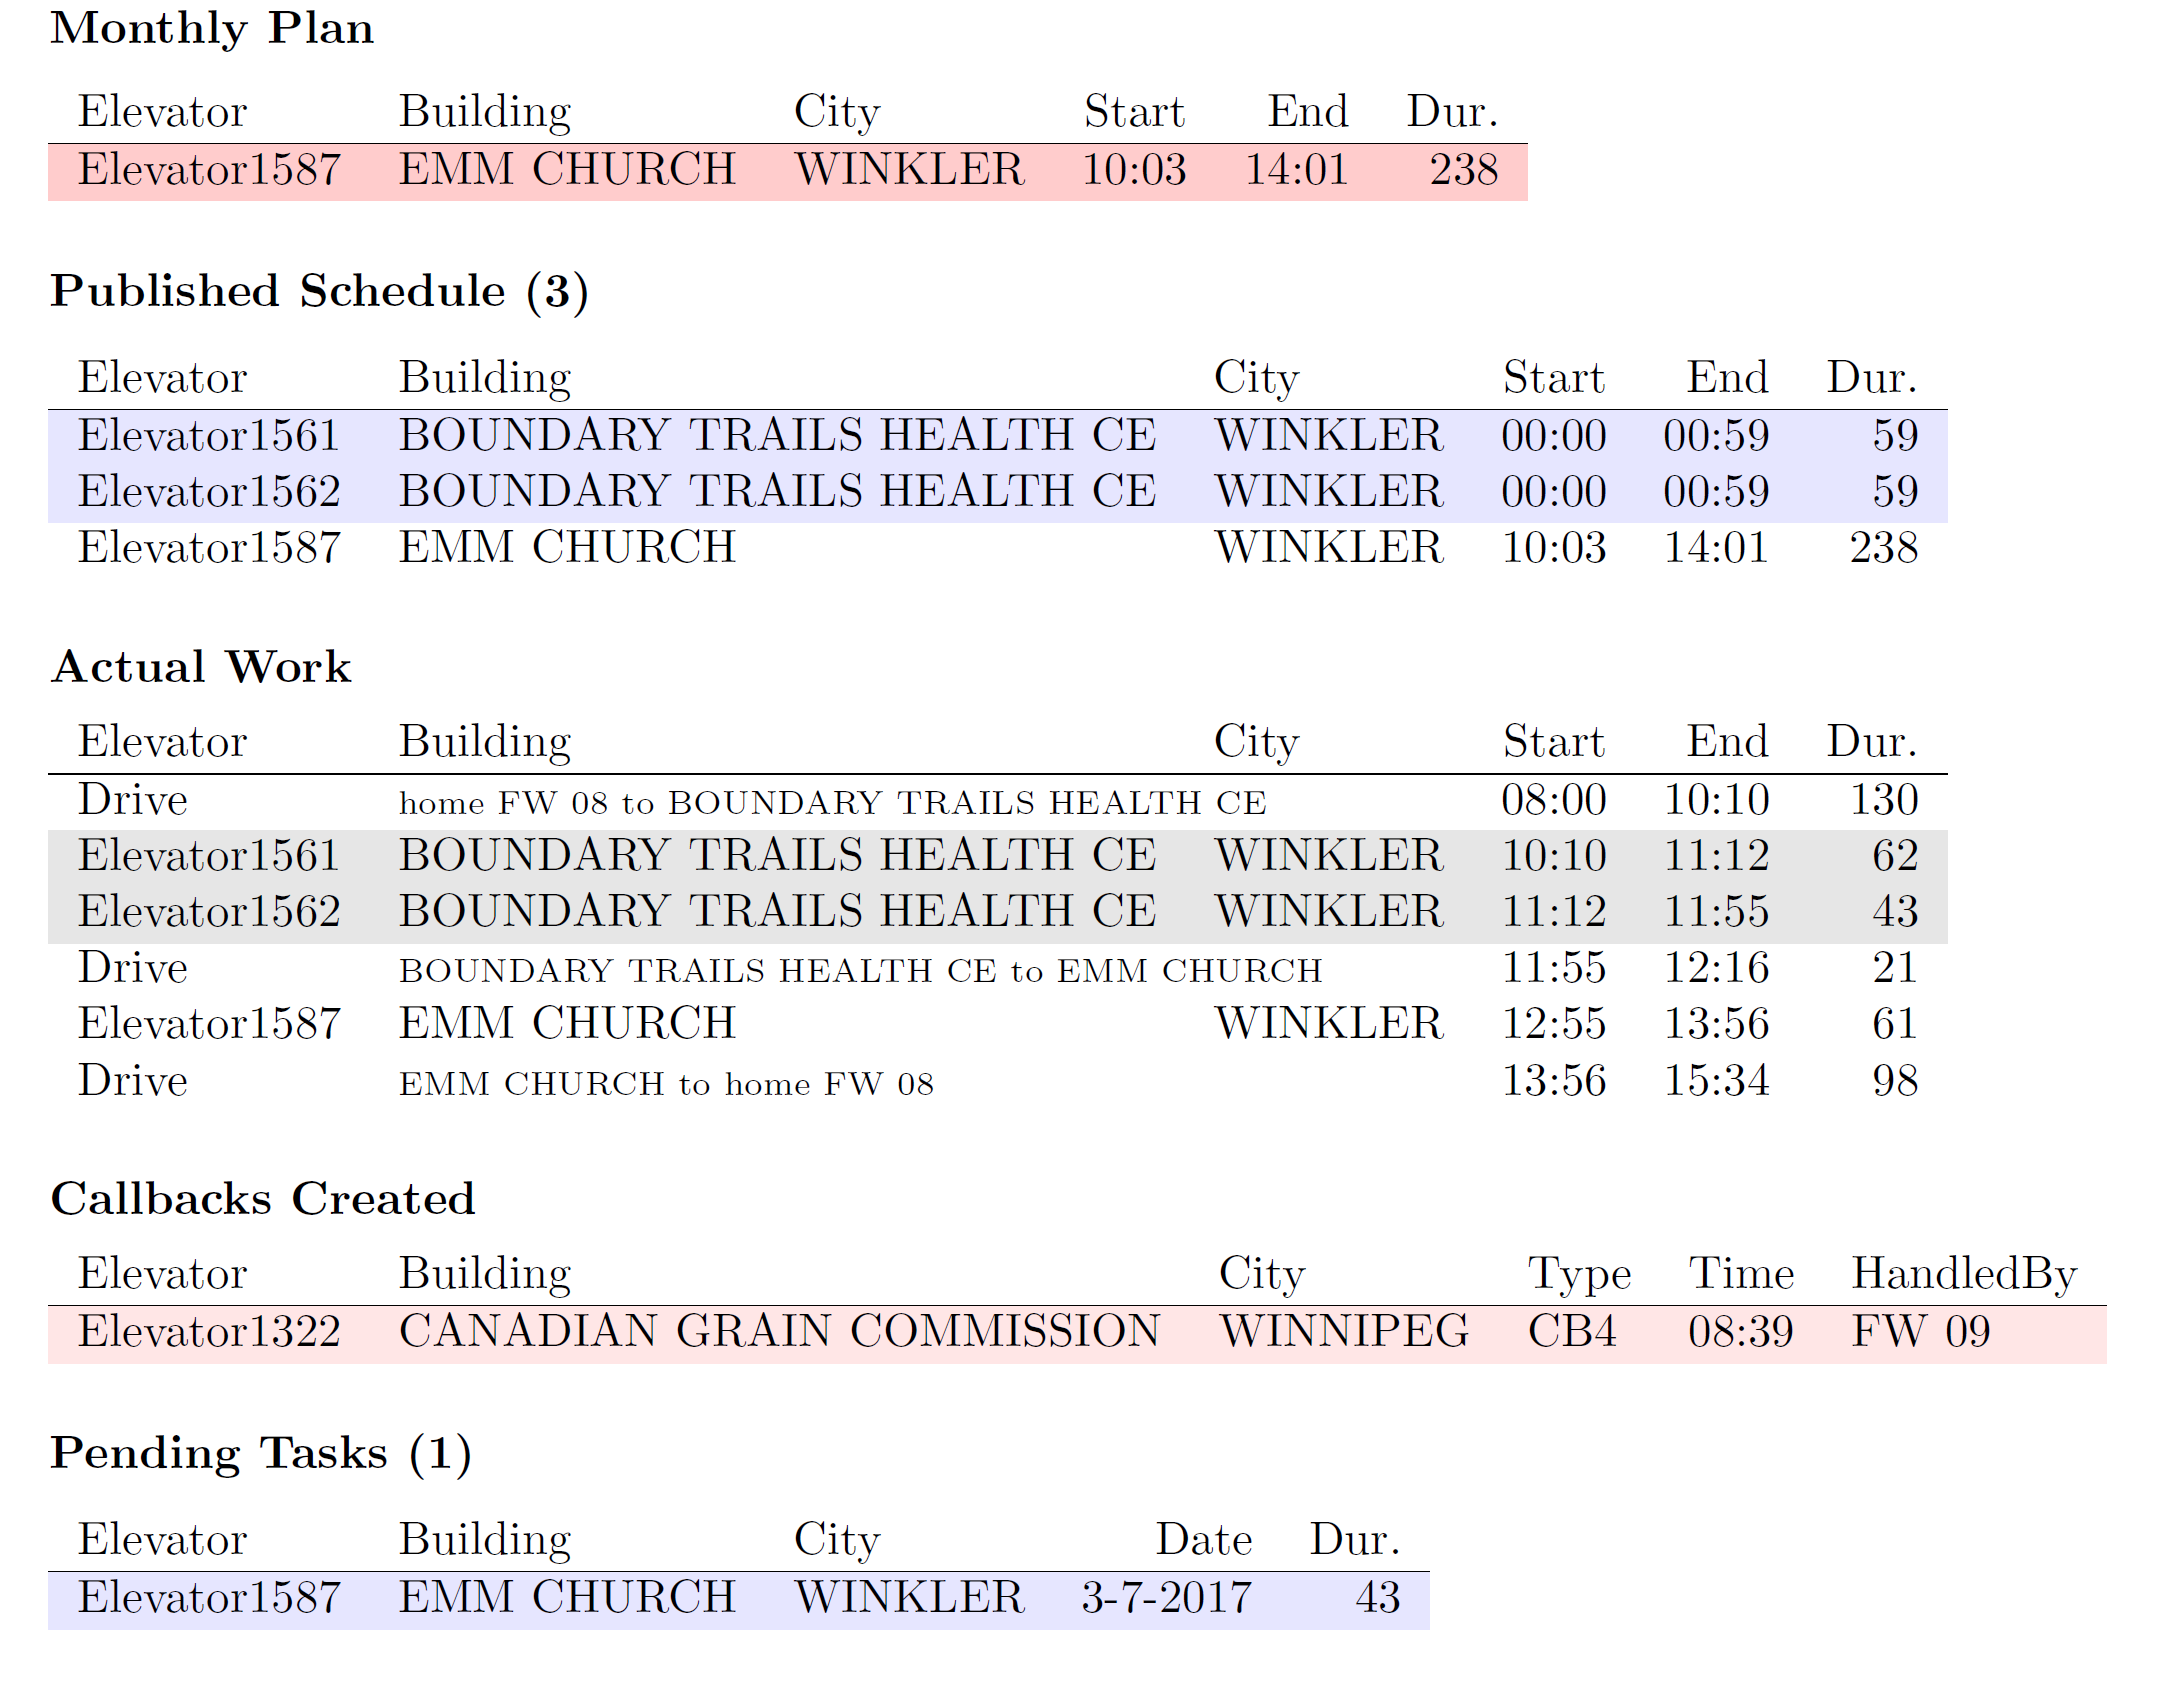
\includegraphics[width=9cm]{imagesfieldservice/detailday}
% \end{frame}

\subsection{Challenges}

\begin{frame}
\frametitle{Challenges: Data}
\begin{itemize}
\item We need company internal data to understand problem
\item Problem for publication, for continued work
\item Open data as alternatives
\begin{itemize}
\item New York City
\begin{itemize}
\item 76,000 elevators with locations
\end{itemize}
\item Toronto, ON
\begin{itemize}
\item 40,000 elevators
\item Inspection dates, outcomes
\item Accident and injury reports
\end{itemize}
\end{itemize}
\end{itemize}
\end{frame}

\begin{frame}
\frametitle{Challenges: Scalability}
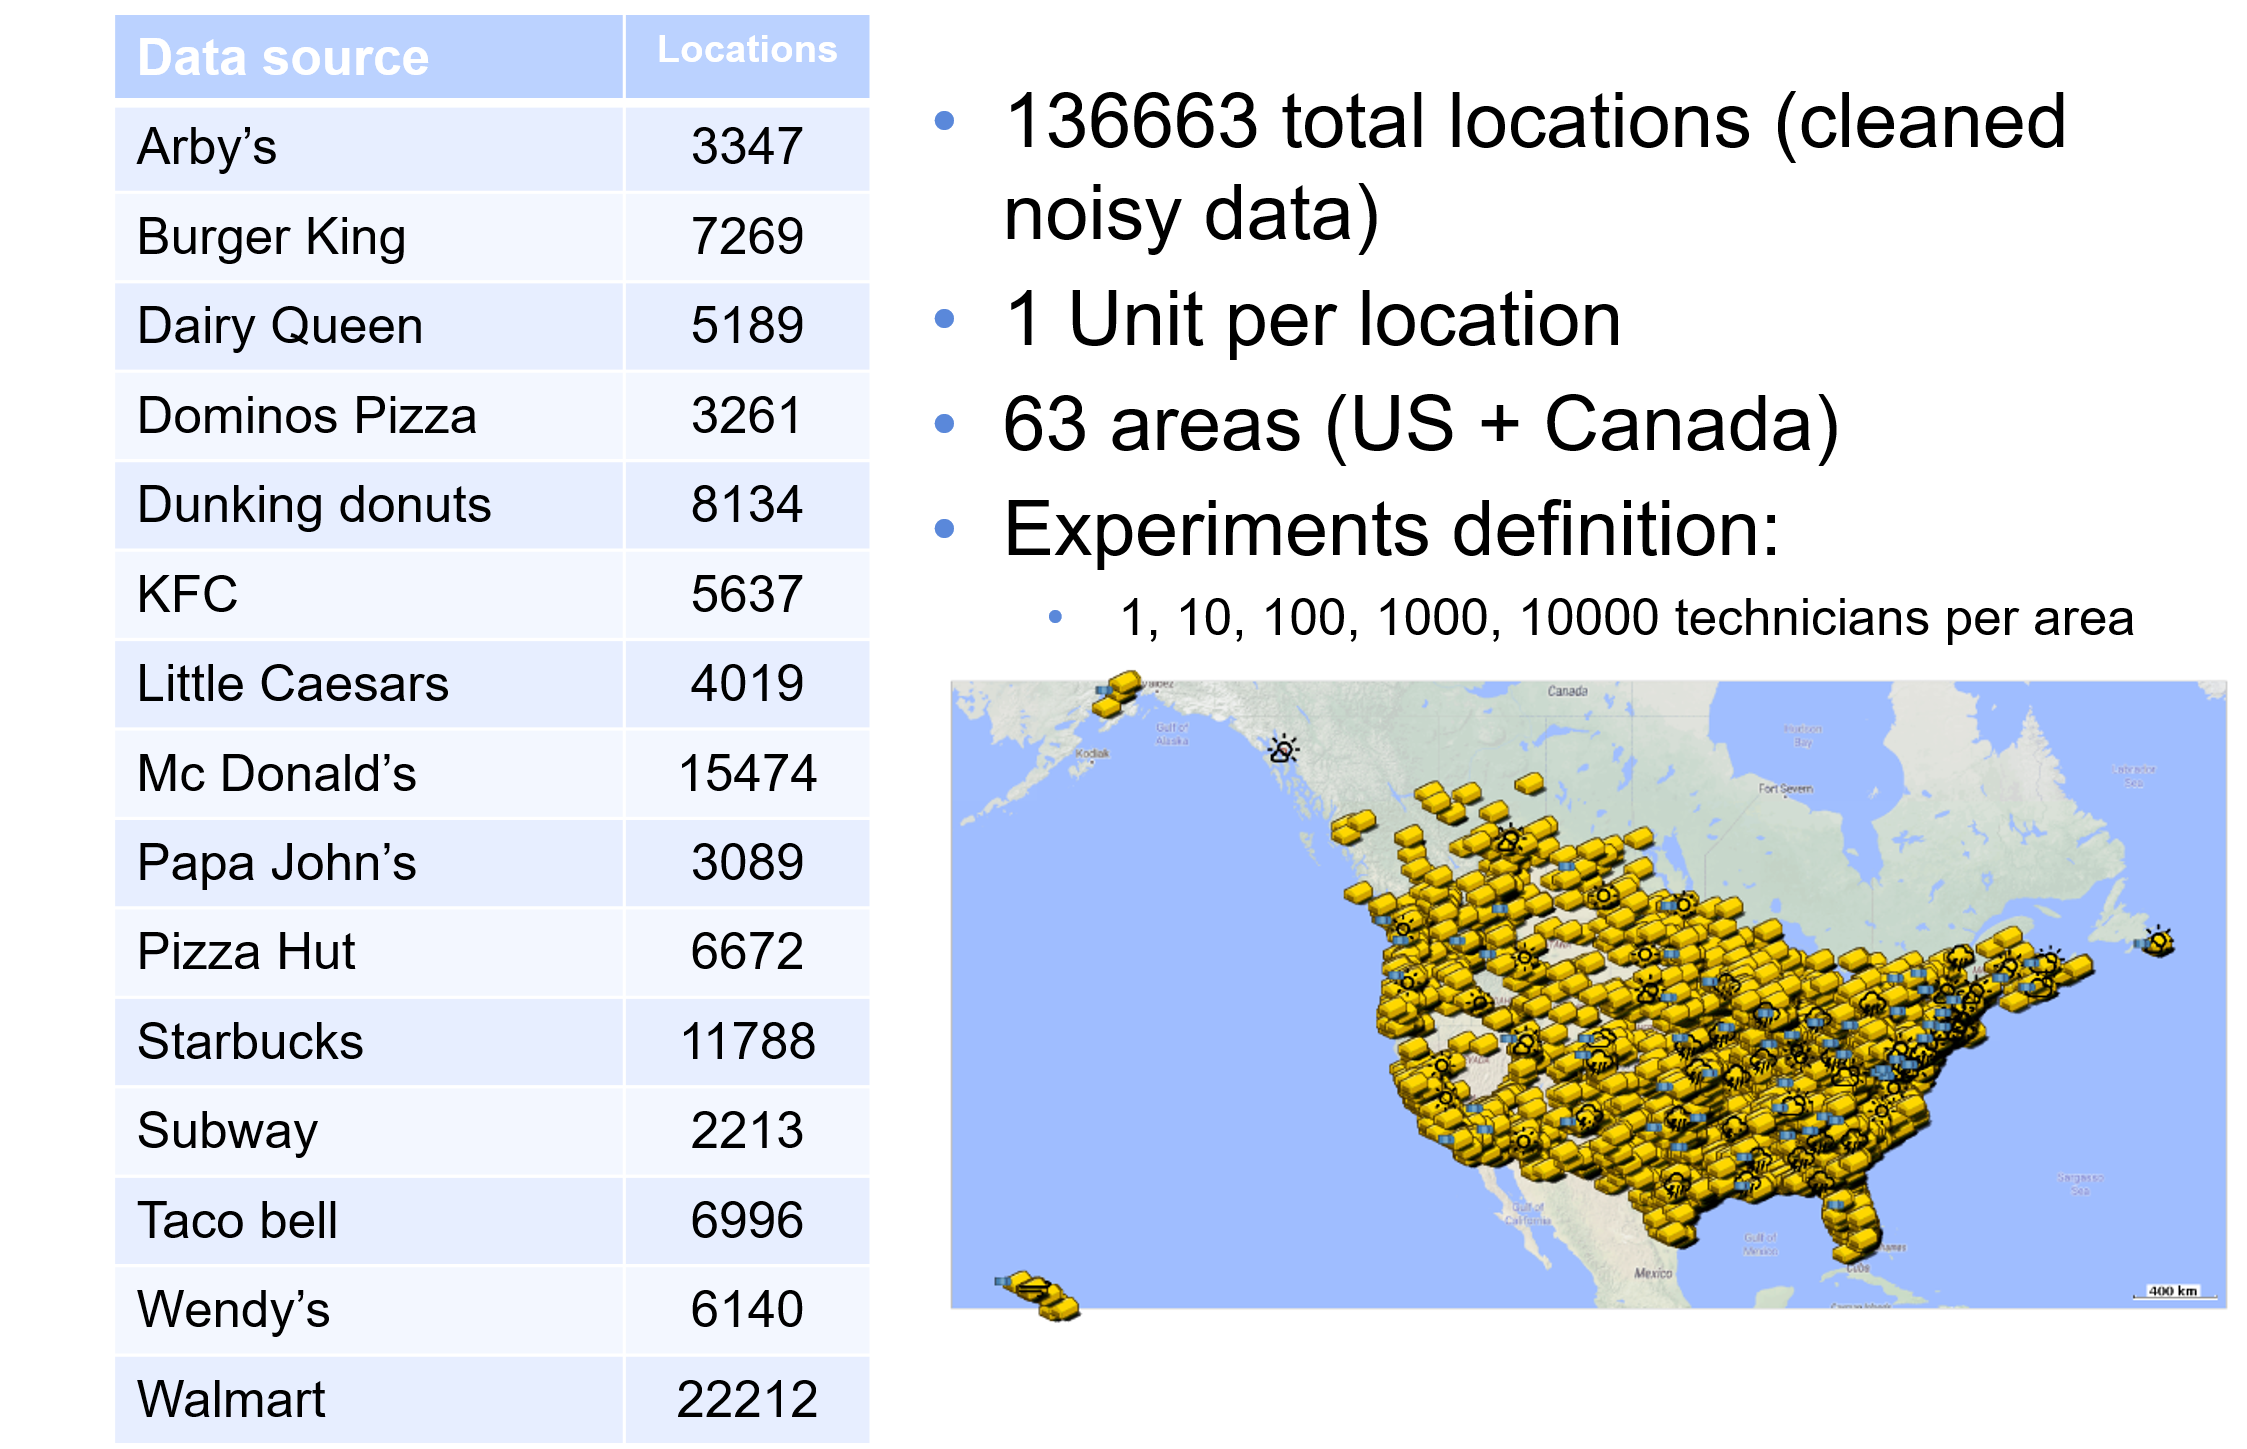
\includegraphics[width=11cm]{imagesfieldservice/simulatorscalability}
\end{frame}

\begin{frame}
\frametitle{Challenges: Tools and Results}
\begin{itemize}
\item We provide research and experimental software
\item \textbf{Not} a solution
\item End-user would like applicable results
\item Managing expectations is important
\end{itemize}
\end{frame}

% \begin{frame}
% \frametitle{What I did not talk about}
% \begin{itemize}
% \item Preferences and Incentives
% \begin{itemize}
% \item Retention of personnel
% \item Optimize while taking preferences into account
% \end{itemize}
% \item Elevator health
% \begin{itemize}
% \item If you don't do the maintenance, then elevators will fail
% \end{itemize}
% \item Condition Based Maintenance
% \begin{itemize}
% \item You can predict some of the failures and prevent them
% \end{itemize}
% \end{itemize}
% \end{frame}


\begin{frame}
\frametitle{Conclusions}
\begin{itemize}
\item We presented the Travelling Repair Person Problem
\item Important as an industrial problem
\item Interesting as a research challenge
\item We use combination of optimization and simulation to deal with novel properties of problem
\item System transferred to customer in 2019
\end{itemize}
\end{frame}
